% to add:
% - the lack of music, ``the silence in [Lumet's] films was not \textit{no} music, it was vérité music." (from whatever happened to great movie music). So consider here the conscious decision to have no music, the implications it has on the "realness".
% - section on diegetic sound, go through original essay (AD comments on Draft 2) and add/expand.
% - Go through A's comments pinned on board


\section{Introduction}

The paranoid thriller is a fundamental genre to 1970s American cinema.
This is due to its overt prioritising of political or corporate conspiracy.
I turn now to my discussion of this genre which, while not unique to the 1970s, has become one of the decade's most recognisable and celebrated trends.
I will discuss here how this genre was shaped by the socio-political climate, and how it represented contemporary anxieties.
In doing so, I will outline how these aspects contribute to the depiction of the American national character through my primary case study, David Shire's score for \citetitle{pakula_all_1976} (Alan J. Pakula, 1976). 
My analysis of this film reveals a subversion of typical political ideologies found in paranoid thrillers given its celebration of the heroic American figure that Turner alluded to. 


\section{\textit{All the President's Men}'s Score}

\subsection{Score Overview}

\textit{All the President’s Men} features a score composed by David Shire; however it is used minimally throughout the film, with non-diegetic music only heard for roughly eight minutes of the film's 133-minute runtime.
The score includes a relatively small ensemble of oboe, contrabassoon, French horn, piano, electric piano, acoustic guitar, electric bass guitar, cello and harp.
At no point do all instruments perform on the same cue.
Rather, even as the score becomes more expansive at later stages of the film, we typically only hear a small ensemble of between two and five instruments.
Shire's non-diegetic cues are typically heard during montage sequences, or when the film veers away from its ``realist,” docudrama aesthetic and more formalist cinematic techniques are utilised.
Each cue typically features droning bass tones, a rhythmic bassline, and a simple melodic motif made up of small intervals. I will discuss these motifs in greater detail below.

Sean Wilson notes in \textit{The Sound of Cinema: Hollywood Film Music from the Silents to the Present} that infrequent placement of music was a common feature of Pakula's trilogy of paranoid thrillers: \citetitle{pakula_klute_1971} (1971), \citetitle{pakula_parallax_1974} (1974), and \citetitle{pakula_all_1976}.
Music's sparsity was key in foregrounding these films' narratives and political critiques.
Wilson thus describes Shire's score as ``a minimalist score of tone and suggestion, almost invoking a hushed sense of dawning realization."\autocites[][119]{wilson_sound_2022}

Shire's conscious avoidance of ``traditional" orchestral scoring and Pakula's conservative use of the score throughout the film, Steven Saltzman writes, ``focused the music on the quieter undertones and dark implications of an unravelling presidential scandal."\autocites[][34]{saltzman_music_2015}
The decision to use the score so rarely throughout the film, as well as to eschew ``snappy cues" and ``noble anthems" often used to evoke presidential symbolism, can clearly be read as an insight into the film's political ideology.\autocites[][34]{saltzman_music_2015}
For although the film celebrates the traditionally heroic attributes of the two protagonists, it simultaneously reflects a disillusionment with myths of heroic American figures and identities, specifically, the nation's president.
This disillusionment is reflected in the score's rejection of overtly traditional ``American" compositional techniques, the likes of which were heard prominently in \citetitle{sherman_big_1971}, for example.
The apparent lack of these elements suggests that the import of the American identity proposed by Turner has faded, an idea that the paranoid thriller often explicitly claimed.
In the place of these traditionally heroic and uplifting cues, Shire's score contributes to the film's discomforting atmosphere through dissonant, sustained and non-diatonic cues.
Furthermore, the decision to avoid conventional Hollywood scoring reinforces the reality of the story being depicted.

To this end, the long stretches of the film that are not underscored with Shire's music are accompanied by a far more ``vérité" style of sound, reflective of the film's docu-drama aesthetic.
The soundtrack is here dominated by diegetic sound effects, most often the sound of typewriters in the \textit{Washington Post} offices.
This wall of noise created by the typewriters contribute towards the film's verisimilitude, and was a conscious decision in order to create the sense that this was a real, functioning newspaper office.\autocites[In order to maximise this sense of realism, Pakula had the crew build an exact replica of the \textit{Washington Post} offices which they ``decorated with trash transported from the real one in Washington."][]{boorstin_its_2016}
As Associate Producer Jon Boorstin wrote, Pakula rejected the ``idea of copying the reality of a certain kind of documentary. … Yes, the audience had to believe. But it also had to be transported."
Pakula ``transports” the audience into the world of journalism by employing several sound recording and mixing techniques that had become common practice during the New Hollywood era, such as characters talking over each other, speaking with their backs to the camera, and naturalist, ambient room sounds.
This extends beyond the newsroom, to outdoor restaurants, office waiting rooms, and witnesses' homes.

The rejection of non-diegetic scoring by directors who favoured an ostensibly more realistic sound was a common source of frustration for many Classical Hollywood composers.
Elmer Bernstein and David Raskin, for example, both authored articles in the early 1970s that lambasted the contemporary state of film composing.
Though Bernstein's and Raskin's ire was predominately focussed on the trend of scoring films with popular music rather than art music, they protested more broadly against the ``dramatic reimagining of musical space in Hollywood films of the early 1970s," as Julie Hubbert surmises.\autocites[][207]{hubbert_whatever_2003}
This included the choice to prioritise diegetic sound effects – even if it meant a scene playing out in silence – and diegetic source music, in order to exacerbate a film's realism.
One director who embraced this way of soundtracking their films was Sidney Lumet, who used this style in \citetitle{lumet_dog_1975} (1975) and \citetitle{lumet_network_1976} (1976), while \citetitle{lumet_serpico_1973} (1973), much like \textit{President's Men}, featured only a very slight usage of non-diegetic scoring.
Hubbert goes on to claim that ``the silence in [Lumet's] films was not \textit{no} music, it was vérité music."\autocites[][195]{hubbert_whatever_2003}
This description can easily be applied to many of Pakula's film and, in particular, \textit{President's Men}.
\textit{President's Men} seems therefore to aspire not just to create a realistic film world, but also to adhere to what had become standard fare in many contemporary films.
I will discuss the significance of foregrounding the diegetic soundtrack and the use of vérité music below.



\subsection{David Shire}

Prior to working on \textit{President's Men}, Shire composed the score for another celebrated paranoid thriller, Francis Ford Coppola's \citetitle{coppola_conversation_1974} (1974). 
This earned him a reputation for composing quiet, minimal scores which he described as ``brain surgery" scores.\autocites[][18]{chattah_david_2015}[David Shire, quoted in][]{budinger_interview_1995}
For these scores, he says he ``made a conscious effort to keep the music out of the way with a score that works largely at an almost subliminal level."\autocites[][18]{chattah_david_2015}
Shire also began to experiment with more modernist practices during this period while remaining stylistically diverse and comfortable composing in different genres and styles.
As Juan Chattah notes in his film score guide for \textit{The Conversation}, Shire's versatility allowed him to thrive at a time when a realignment of composers' roles within the film industry saw them transition from contracted to specific studios to independent freelancers.\autocites[][23]{chattah_david_2015}[Caryl Flinn also discusses this shift in composer contracts, and I will explore this in more detail in the following chapter during my analysis of \textit{Alien}.][]{flinn_strains_1992}
In addition to his work in more dramatic narrative films, Shire also worked in musical theatre and musical films, further demonstrating his versatility and capacity to work across different mediums, styles, and genres.

Examples of Shire's diverse compositional styles can be heard in his scores for \citetitle{sargent_taking_1974} (Jospeh Sargent, 1974) and \citetitle{richards_farewell_1975} (Dick Richards, 1975).
In \textit{Pelham 123}, Shire took influence from Alfred Schoenberg's twelve-tone technique and composed a modernist jazz score which reflected urban New York in the 1970s.
In \textit{Farewell}, he composed a big band score which was largely era-appropriate for the film's 1940s setting.
The film's exploration of the fading importance of protagonist Philip Marlowe's ethics and values was complemented by extended instrumental performance techniques.
In \textit{President's Men}, meanwhile, Shire largely adhered to far more conventional instrumental techniques and restrained melodies and rhythms, thus appropriating Pakula's austere, conservative filmmaking.
The extent to which Pakula embraced this form of filmmaking for \textit{President's Men} caused Shire to question the need for any music at all in the film.
He stated his concerns in an interview from the 1976 episode of the radio show ``Cinema Showcase" that aired two months after the film was released:
\begin{quote}
when they first contacted me about doing the score, and I saw the picture a couple of times, I told them that they really, probably needed no music at all. … It has a kind of documentary realism in places that made it difficult for me to think of what kind of music could go with the picture without breaking the mood of it and making it sound like we were trying to artificially hype it.\autocites[][]{schwartz_cinema_1976}
\end{quote}
Despite his concerns in this instance, Shire has otherwise stated that his objective when scoring films is to create a subtle and ambiguous accompaniment to the onscreen action.
When asked what he found the ``most satisfying use of music in a film," he answered,
\begin{quote}    
film music is so often an art of juxtaposition. When the music is more about subtext–adding an element that isn't on the screen–that's the most satisfying. ... The fun is when the score can find an element that weaves into the whole mix–if there's a love scene, instead of making it just more loving, there's an underlying tension. So the melody is saying ``love" but there's something underneath that's saying, ``Wait a minute, there's something \textit{else} going on here." There's an ambiguity about it.\autocites[David Shire, quoted in][1]{morgan_knowing_2000}
\end{quote}
Shire's attempts to both complement and complicate the onscreen action led to him describing his music as ``\textit{Gebrauchsmusik}."\autocites[][23-24]{chattah_david_2015}
As described in the \textit{Historical Dictionary of Modern and Contemporary Classical Music}, \textit{Gebrauchsmusik} ``renounced art-for-art’s-sake,” though it is more generally understood as music composed for a specific purpose, and should not be removed from the context for which it was intended.\autocites[][]{gagne_historical_2012}
By his own admission, Shire's scores are therefore intrinsically tied to the narrative they were composed to accompany.
He acknowledged this in a 2004 interview:
\begin{quote}
Some of my most effective scores and cues will never be performed at a pop concert and will not sound very interesting away from the movie. But they had to be that way. Take much of the score for \textit{All the President's Men}. Played away from the movie you'd fall asleep in five minutes. But the job wasn't to write pop concert themes or a soundtrack album. The job was to help make that movie play as well as it could.\autocites[][15]{armstrong_high_2004}
\end{quote}
He touched upon this point in the ``Cinema Showcase" interview, claiming that it was ``impossible" to release \textit{President's Men}'s score as an album, although his point here is more about the amount of music used rather than the style of music itself.\autocites[][]{schwartz_cinema_1976}


As Gerald Mast writes in his \textit{A Short History of the Movies}, the 1960s and 70s saw a decline in traditional Hollywood conventions of scoring ``a scene with music that increases the action's emotional impact without making the viewer aware of the music's existence." (Mast420 - check year)
Shire's philosophy and approach to film scoring, in tandem with his stylistic diversity therefore fit well within this period, as composers tended away from traditional, symphonic orchestral scoring.
This trend suited Shire's preference to elicit more ambiguous emotional registers through less melody-oriented scores, while his comfort composing symphonic- and musical theatre-inspired milieus simultaneously afforded him opportunities within more mainstream and conventional films.





\section{Paranoid Thriller Overview}

As I alluded to above, the paranoid thriller did not entirely originate in the 1970s.
Yet, although it has multiple antecedents from throughout the history of cinema – film critic R. Barton Palmer provides an overview of the genre's debts to Alfred Hitchcock, for example – it is deeply tied to the political climate of its era.\autocites[][85-108]{palmer_hitchcock_2006}
I detailed much of this political climate in my introduction, but it is important to reiterate the seismic impact that this period had on the nation's psyche when discussing certain elements of Shire's score for \textit{President's Men}.

To fully appreciate the significance of paranoid thrillers it is important to acknowledge the impact of the Vietnam War.
The war naturally had a major impact on the nation, and a major political rift emerged, arguing for the war's righteousness or illegitimacy.
And yet, during the war itself, only one narrative film was released that was specifically about the war: \citetitle{wayne_green_1968} (1968), a film directed by and starring John Wayne, who championed its production to counter the growing anti-war sentiment throughout the country.
Despite the dearth of films addressing the war itself during the USA's involvement, film critic Pauline Kael claimed that ``Vietnam we experience indirectly in just about every movie we go to ... because we're all tied up in knots about that rotten war."\autocites[][35]{lerman_pauline_1996}
The war's legacy can be found in a number of films of the era that, Kael claims, ``are based on American self-hatred."\autocites[][35]{lerman_pauline_1996}

With regards to paranoid thrillers, this legacy, and the source of self-hatred, pertains directly to the revelations that the government had been concealing many of their actions during the war.
When the full extent of the war's reach was revealed to the public following the controversial leaking of the ``Pentagon papers," the nation was faced with what Christian Keathley identifies as ``the onset of trauma resulting from a realisation of powerlessness in the face of a world whose systems of organisation – both moral and political – have broken down."\autocites[][293]{keathley_trapped_2004}
The war was arguably the most consequential event of this period, yet the trauma that Keathley identifies was an effect of multiple events that shook the political and societal landscape, including, but not limited to:
the assassinations of President John Kennedy, Robert Kennedy, Malcolm X and Martin Luther King;
the Watergate scandal;
anti-war, civil rights, and gender equality protests, and the violence that often followed;
urban riots;
the OAPEC oil crisis;
and a bribery scandal concerning Vice President Spiro Agnew.
These events and the trauma they inflicted instilled a deep sense of paranoia and cynicism that heavily inspired, and came to be almost synonymous with, the New Hollywood period and the Seventies Film.
As Jonathan Kirshner lays out, paying particular mind to Watergate, these events brought about ``the collapse of faith in institutions, a foreboding sense of the erosion of privacy, and a basic loss of trust, in one's president, in one's colleagues, and in one's (presumed) friends.”\autocites[][135]{kirshner_hollywoods_2012}
David Cook echoes Kirshner's claim, highlighting the historic significance of this period's existential trauma: ``the American public lost faith in its institutions as never before."\autocites[][116]{cook_1974_2007}
This lack of faith and security was so pervasive during this period that \textit{The Conversation}, one of the most celebrated and iconic paranoid thrillers of the era, was actually written before the revelations of the Watergate scandal which later proved to be one of the genre's most important catalysts.
It was within this context that the paranoid thriller arose.

Conspiracies and cover-ups can be found throughout many films in the 1970s. 
Some films were overtly about such conspiracies – such as \citetitle{pakula_parallax_1974} and \citetitle{polanski_chinatown_1974} (Roman Polanski, 1974) – while others hinted at it more allegorically – such as \citetitle{spielberg_jaws_1975} (Steven Spielberg, 1975) and \citetitle{guillermin_towering_1974} (John Guillermin, 1974), both of which featured nefarious corporate interests that put innocent lives at risk.
Many paranoid thrillers follow similar trends.
However, the plots themselves, and therefore their subtextual critique, often differ greatly.
Regardless of the plot specifics, they typically focus around a single individual who seeks to uncover a plot by a villainous private company or rogue governmental operatives.

These films responded to contemporary fears that governmental overreach, and unregulated and unscrupulous corporations kept the nation's citizens under close surveillance.
These fears extended to the idea that citizens' individual freedoms were under threat, while those in power were willing to murder those who threatened their authority.
As such, what is often at risk in these films is the sanctity of the national identity, the notion that within a late-capitalist society, it is becoming increasingly difficult to maintain one's individualist autonomy and self-sufficiency.

A succinct description of the typical paranoid thriller can be found in Robin Wood's discussion of the films of Robert Altman: ``the protagonist embarks on an undertaking he is confident he can control; the sense of control is progressively revealed as illusory; the protagonist is trapped in a course of events that culminate in disaster (frequently death)."\autocites[Although Wood here is referring specifically to the films of director Robert Altman, who did not direct any paranoid thrillers, his summation perfectly mirrors the paranoid thriller. This can be seen as justification of the claim that this is perhaps the quintessential genre of the period, and a perfect crystallisation of the paranoia and disillusionment that apparently encapsulated the era.][27]{wood_hollywood_1986}
These existentially downbeat endings read as a mourning of the loss of individuality, a cornerstone of the American identity, in addition to the decline of patriarchal domination.

Yet, while these films end with their protagonists realising the futility of fighting the powers-that-be (\citetitle{polanski_chinatown_1974}, \citetitle{coppola_conversation_1974}), overcoming their antagonists only to realise their ultimate insignificance and powerlessness (\citetitle{pollack_three_1975}, \citetitle{pakula_klute_1971}), or even dead (\citetitle{pakula_parallax_1974}), \citetitle{pakula_all_1976} present a far more optimistic narrative.


\section{\textit{All the President's Men}}

Director Alan J. Pakula was one of the directors most closely associated with 1970s paranoid thrillers, specifically due to his ``Paranoid Trilogy": the aforementioned \citetitle{pakula_klute_1971}, \citetitle{pakula_parallax_1974}, and \citetitle{pakula_all_1976}.
The plots of these three films differ greatly.
And yet, they share similar subtexts and ideologies, summarised film critic Chris Vognar: each film ``take[s] for granted that important people are lying, and, in some cases, killing to cover it up."\autocites[][]{vognar_parallax_2021}
Ian Scott, in his book \textit{American Politics in Hollywood Film}, similarly notes this while referencing the trilogy's impact and legacy:
``Pakula's films provided the thread for an examination of American politics and society from beyond authority and accountability in the 1970s and in the process created cinematic form and content that would define the agency of paranoia cinema in its entirety."\autocites[][138]{scott_american_2011}

Despite this thematic similarity, however, \textit{President's Men} differs from Pakula's earlier films in its depiction of what Robert Torry might define as a ``therapeutic narrative.”
Torry defines such narratives as seeking to challenge the ``sense of essentially impotent outrage and despair" that was commonplace during the Vietnam era.\autocites[][27]{torry_therapeutic_1993}
Torry focuses on \citetitle{peckinpah_wild_1969} (Sam Peckinpah, 1969) and \textit{Jaws}, and defines these films as attempts to ``diagnose and propose a remedy for the national trauma of the Vietnam era."\autocites[][27]{torry_therapeutic_1993}
This description proves accurate for \textit{President's Men}, wherein the two protagonists strive to ``[re-establish] the mythically moral and political rectitude of the American antifascist enterprise."\autocites[][34]{torry_therapeutic_1993}




\subsection{Narrative Overview}

\citetitle{pakula_all_1976} tells the true story of \textit{Washington Post} journalists Bob Woodward and Carl Bernstein as they attempt to uncover the truth behind the 1972 break-in at the Democratic National Committee's headquarters in the Watergate hotel.
The film opens with the break-in itself: five men in suits are seen sneaking into the hotel but are soon caught and arrested.
Woodward is assigned to report on the burglars' arraignment the next day.
At first he assumes the story of little significance but, after learning that one of the burglars is a former CIA employee, Woodward begins to investigate the case further.
Along with his partner, Bernstein, Woodward discovers that the break-in was ordered and orchestrated by the Campaign to Re-elect the President (CREEP) and President Richard Nixon himself.

Throughout the film, we see Woodward and Bernstein as they investigate the story by interviewing multiple current and former employees of the administration, and attempt to piece the story together.
In addition to multiple anonymous sources, Woodward is guided by the mysterious figure ``Deep Throat," the then-unnamed source who was later revealed to be Deputy Director of the FBI Mark Felt.
His meetings with Deep Throat take place in a deserted car park late at night, providing an ominous and disquieting setting in direct contrast to the brightly lit newspaper offices and the witnesses' homes that the majority of the film takes place in.
This setting, and Deep Throat's revelations that the reporters lives are in danger, provide the film with a direct menace that aligns the film with similar paranoid thrillers in which the protagonists' investigations endanger their lives.

Unlike most paranoid thrillers, however, \textit{President's Men} tells a true story, albeit one with fictionalised elements.
As such, rather than representing the nation's trauma through fictional antagonists, it presents a literal representation of the corruption and the abuses of power that fundamentally shook the nation's psyche.
In its depiction of a widespread, criminal conspiracy, led by those at the very top of the United States’ government, \textit{President’s Men} gives us an insight into exactly \textit{why }the nation was justified in feeling a sense of ``disaffection, alienation, and demoralisation.”\autocites[][296]{keathley_trapped_2004}
It subsequently seeks to provide a remedy for this disillusionment by presenting a narrative in which its protagonists are able to successfully bring down the malevolent forces responsible.


\subsection{\textit{All the President's Men}'s Themes} \label{sec:president-themes}

\textit{All the President's Men} was widely acclaimed upon its release.
One reviewer, Louise Sweet, wrote in the BFI's \textit{Monthly Film Bulletin} that the film challenges ``the sense of power being mythologised and rendered invincible."\autocites[][95]{sweet_all_1976}
In this sense, \textit{President’s Men} is a film about the process of de-mythologisation of the righteousness, trustworthiness, and morality of the US government, and depicts \textit{how} such myths are upended. 
This idea is made explicit by Deep Throat when he tells Woodward to ``forget the myths the media’s created about the White House. The truth is these are not very bright guys” (00:38:29).


We can understand \textit{President's Men} to some extent as a quasi-revisionist film, as it addresses longstanding myths surrounding the nation's self-perceptions – specifically those regarding the government's infallibility – and highlights the true wrongdoings of those in power.
Critical evaluation of the mythologisation of the US and its history is typically understood as a liberal undertaking.
\textit{President’s Men} nevertheless depicts a number of more conservative filmic tropes.
Specifically, in the characters of Woodward and Bernstein, as the film points to the necessity of strong and ethical male heroes to uphold a series of moral and legal codes.
Terry Christensen discusses this, writing that the film’s message is ``politics is corrupt and that bad men can gain great power, but it also said that brave individuals, a free press, and public opinion can bring the evil men down."\autocites[][134]{christensen_reel_1987}
That the ``brave individuals” in this case are real people and not fictional characters, the film’s dichotomous undertaking of dispelling US mythology and celebrating individualist triumphs and American heroes is complicated, as Carl Bernstein and Bob Woodward are essentially placed within the pantheon of ``Great American Heroes.”
Jon Boorstin made this connection when he noted that ``the point of the movie is that these guys are unstoppable … they’re a force of nature and they’re going to save the world.”\autocites[Boorstin, quoted in][]{hornaday_how_2022}
Pakula is likewise quoted in Mark Feeney’s \textit{Nixon at the Movies}, wherein he acknowledged Woodward and Bernstein as righteous heroes, apparently failing to note any complexities in simultaneously anointing them as heroes while also questioning mythologies surrounding the United States:
\begin{quote}
it’s inherent in the story of Carl and Bob that they have become a kind of contemporary myth [whose experience affirms] that American belief that a person or small group can with perseverance and hard work and obsessiveness take on a far more powerful, impersonal body and win – as long as they have truth on their side.\autocites[Pakula, quoted in][256]{feeney_nixon_2004}
\end{quote}
Pakula thus aligns Woodward and Bernstein with the heroic American ideal that Turner celebrated, while simultaneously presenting what Christensen described as ``the traditional Hollywood view" of the strong individualistic hero.\autocites[][134]{christensen_reel_1987}
He further made this explicit in a quote printed in \textit{Entertainment Weekly} article wherein he claims that, while \textit{The Parallax View} ``destroyed the American hero myth ... \textit{All the President's Men }resurrects it."\autocites[Pakula, quoted in][]{aquilina_all_2021}

Woodward and Bernstein neatly fit within Michael Ryan and Douglas Kellner’s notion of the ``individualist male hero,” a figure that they claim became commonplace within late 1970s and 1980s American cinema.\autocites[][15]{ryan_camera_1988}
These heroes, Ryan and Kellner argue, demonstrate three key ideals:
they are warriors who ``buck government power and stand up to state tyranny”;
they are entrepreneurs, in that they are demonstrate a ``callousness and … survivalist mentality of the market”;
and they are patriarchs, ``who [dominate] women.”\autocites[][219-220]{ryan_camera_1988}
Each of these characteristics respond to Turner's thesis, and align Woodward and Bernstein with Turner's patriarchal American ideology.

Key to the representation of these patriarchal figureheads is the film's placement of women, whose roles are largely defined by their personal or professional relationship to men.
Film historian Michael Cramer discusses this further, highlighting Woodward and Bernstein’s ``seduction … deception … and outright use of force” to gather information from female sources.\autocites[][196]{cramer_neoliberal_2022}
Two scenes in particular exhibit this:
one in which the reporters encourage a female colleague to arrange a date with a former romantic partner who works at CREEP to elicit information (00:59:15);
another when Bernstein visits the home of a female CREEP bookkeeper, invites himself inside, ignores her requests that he leave, and harasses her until she answers his questions (01:10:47).
Cramer continues: 
\begin{quote}
    what is at stake is the women’s commitment to another man, from whose sway she must be freed. … The disturbing scenario here is one in which these women are finally allowed to speak, to break out of the closed and secretive conspiracy and become part of the new, transparent one, in which their `voice’ is liberated, but only so that it may be instrumentalized.\autocites[][196]{cramer_neoliberal_2022}
\end{quote}
Nevertheless, some have read \textit{President's Men} as a means to upend the stability of the patriarchal status quo that Turner's thesis championed.

Elizabeth Kraft, for example, has argued that \textit{President’s Men} is ``basically a `woman’s film,’ a suitable genre in which to address the deep distress suffered by the nation at the discovery of presidential (patriarchal) betrayal.”\autocites[][31]{kraft_all_2008}
For Kraft, woman’s films ``offered the woman viewer the chance to purge frustration at her lot in life through vicarious identification with a victimized, suffering female.”\autocites[][31]{kraft_all_2008}
Molly Haskell offers a far more critical definition, however, opening her essay on the genre by posing a question that highlights the inherently sexist sociocultural environment that has allowed the term to become commonplace:
``what more damning comment on the relations between men and women in America than the very notion of something call the `woman’s film’?”\autocites[][20]{haskell_womans_1999}
She goes on to note that the term ``woman’s film" ``carries the implication that women, and therefore women’s emotional problems, are of minor significance,” and flags the gendered double standard of not referring to ``a film that focuses on male relationships [as a] `man’s film’."\autocites[][20]{haskell_womans_1999}
Anna Bogutskaya also references this when exploring what she terms the ``Angry Woman” character model: ``it’s never called a subgenre when it’s about white male rage – it’s just cinema.”\autocites[][141]{bogutskaya_unlikeable_2023}

As Haskell suggests, ``women’s emotional problems” are often a key facet of woman’s films and are therefore often referred to as ``weepies,” while both Haskell and Kraft note that the genre is closely aligned to daytime soap opera television.
The popularity of these soap operas, Kraft notes, was usurped in 1973 as the Senate Watergate hearings were televised which ``invoke[d] … the emotional distress caused by betrayal, lies, cheating, and arrogant disregard for the rights and feelings of others – the distress, in other words, typically examined and cathartically exorcized in soap operas or in the melodramatic `woman’s film’."\autocites[Kraft refers to several features and set pieces that place \textit{All the President's Men} ``in soap opera territory.” For example, the casting of Nicholas Coster, an actor known from the soap opera \textit{Another World}, as the lawyer Markham; the interaction between Markham and Bob Woodward as the lawyer plays dumb in response to the reporter’s questions (00:07:40); and the flirtatious interview Bernstein conducts with a potential source, Sharon Lyons (00:22:26).][31-34]{kraft_all_2008}
This, along with the underlying themes of betrayal, corruption and secrecy, contributes to the understanding of the film as a melodrama and a woman’s film, wherein both the ``president’s men” and the reporters 
\begin{quote}
are complicit in the creation of a corrupt world in which confidence, sympathy, and trust between individuals are no longer possible. Looking through a woman’s eyes, there is not a lot of difference between the way Nixon’s men sought out secrets and played tricks in the interest of what they conceived of as a higher good … and the measures Bernstein and Woodward employ in pursuit of their higher good.\autocites[][35]{kraft_all_2008}
\end{quote}
If understanding \textit{President’s Men} as a woman’s film, one may assume that it privileges the perspective of the female characters.
However, many of the aspects discussed by Kraft that align it with the woman’s film genre also point to the subjugation of women beneath more powerful male figures.
It is worth noting here that the female figure who perhaps wielded the most authority over Woodward and Bernstein’s reporting, the \textit{Washington Post}’s publisher Katharine Graham, is physically absent from the film and is only referred to by its male characters.



The film therefore clearly displays a conservative masculinity and individualist narrative, in addition to more ``classical Hollywood” traits, defined by Cramer as ``the motivated protagonist, goal-oriented narrative, effective action and overcoming of obstacles, clear conclusion or `happy ending,’ all in the support of an affirmative ideological function."\autocites[][180]{cramer_neoliberal_2022}
The film depicts each of these traits to some degree.
And yet, they are upended somewhat by Woodward and Bernstein’s morally-dubious methods; their ``ideological function,” although justified by their hunting of criminal activities within the White House, appears largely motivated by their own careerist aspirations – evidenced in their glee when stumbling upon breakthroughs in the case.

While \textit{President’s Men }has been the focus of many studies, its soundtrack remains largely unexamined.
I will now turn to this aspect of the film and explore how its soundtrack contributes to the film’s depiction and celebration of aspects of the American identity.

\section{ Soundtrack Analysis}

Analysis of the film's score reveals several recurring motifs which are heard at various points in the film.
Figure \ref{fig:president-all-motifs} showcases these motifs in order that they appear in the film, most of which can be heard at multiple points in the film.
In addition to these motifs but not transcribed in this figure are pedal bass tones and sustained notes in melody lines which are heard in several cues and provide a discomforting sense of dread.
The motifs are often heard played by different instruments and in different keys.
In this figure, though, they are all presented in the shared key of C major.
Despite all opening on C, though, many of the motifs feature non-diatonic notes.
When played alongside other motifs, this non-diatonicism creates a sense of dissonance and make the cues tonally ambiguous, adding to the film’s suspenseful atmosphere.

Although the cues are heard in several different keys, the motifs are used in a mode-preserved transposition of the versions transcribed in this figure.
Some of the motifs, however, are heard with slight variations.
These amended motifs have been arranged in the same row as the version that is originally and most often heard.

The cues throughout the film are built from a number of these motifs in different orders and combinations. 
More motifs are added to these combinations as the film progresses, overlapping with each other and expanding the soundtrack.
The convoluted, layered nature of the reporters' investigation is hinted at by this gradual instrumental layering of the score: as each instrument is introduced, a further layer of the scandal is alluded to.
\begin{figure}
    \centering
    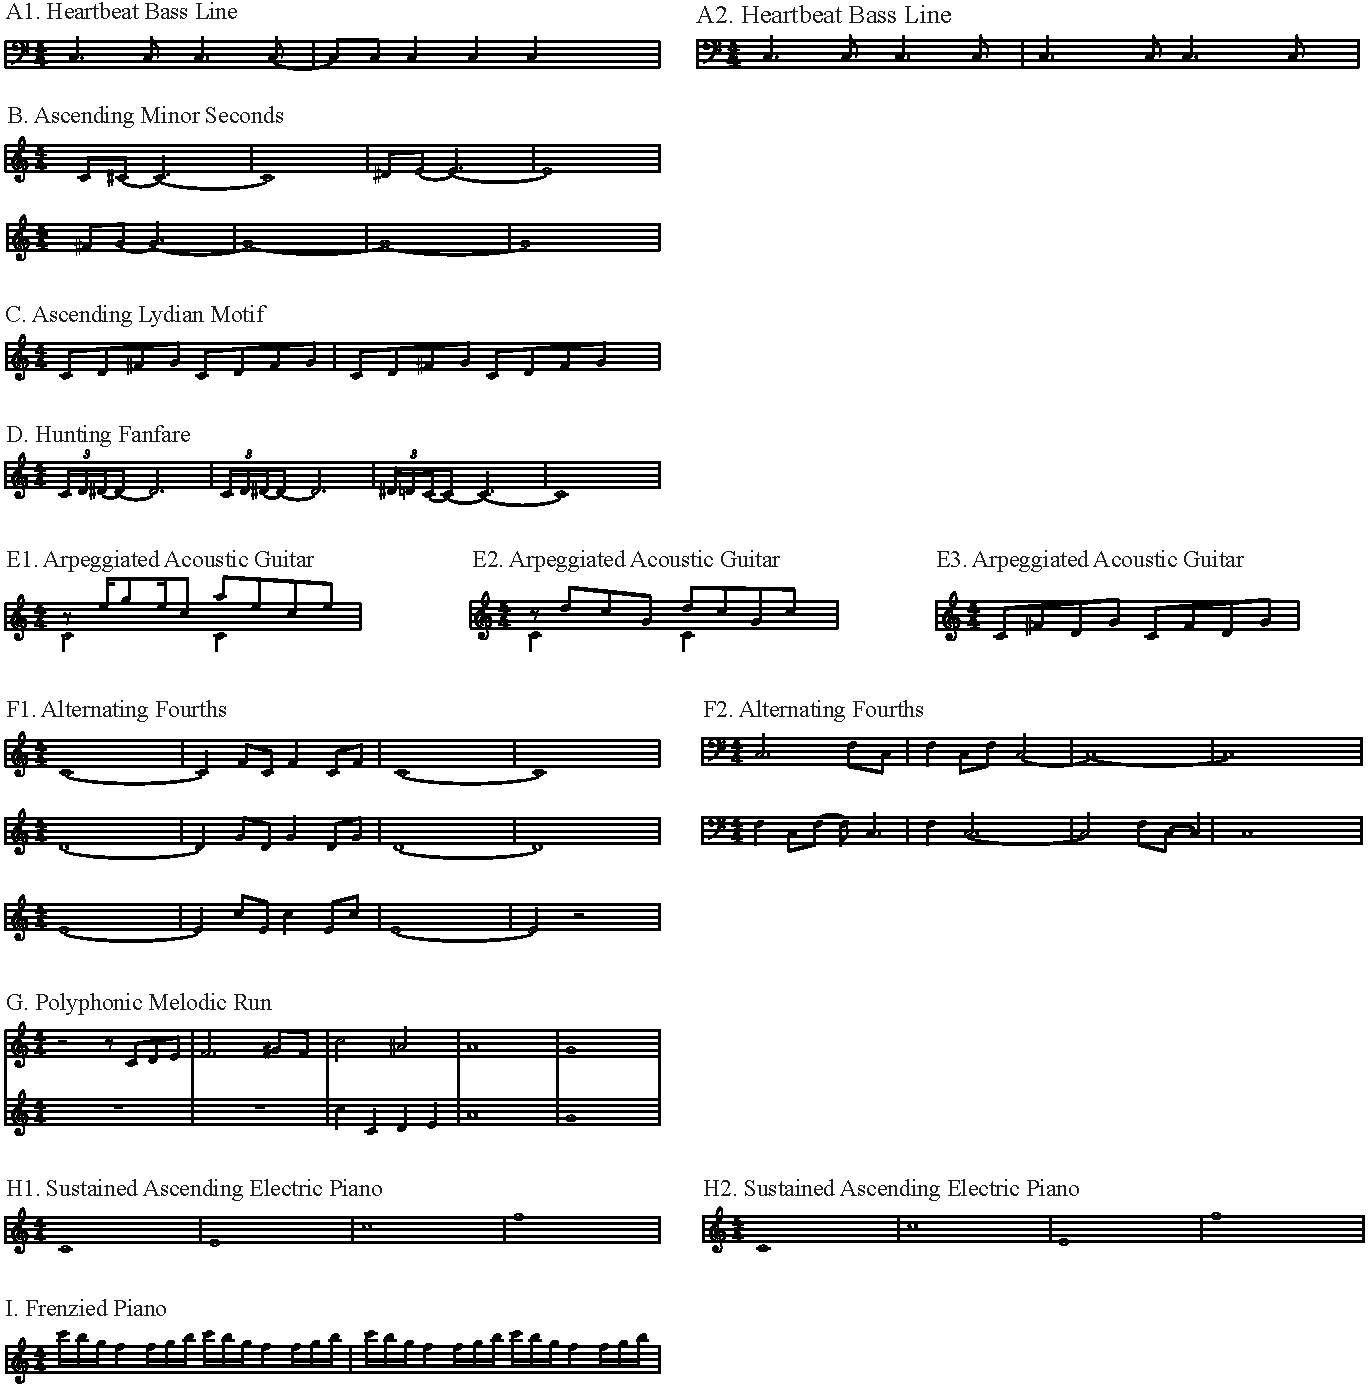
\includegraphics[width=1\linewidth]{img/president-all-motifs.pdf}
    \caption{Transcriptions of motifs heard at various stages of \textit{All the President's Men}. Note that these motifs have all be transcribed in C natural, but are heard in different keys throughout the film.}
    \label{fig:president-all-motifs}
\end{figure}



Before moving on to discuss how these motifs are heard in the film, I will now give a brief analysis of some of the most common motifs to ascertain what they contribute to the film’s political themes.

% Given the relative lack of musical cues in the film, I will now go through each instance of extradiegetic scoring to examine how the music is employed and what we can understand it to be saying about the American identity and ideology. 
% In doing so, I will highlight instances where the film's apparent lamenting of the demise of the celebrated American characteristics can heard.
% This analysis will also reveal perhaps more surprisingly uplifting perspectives of this American identity during what President Gerald Ford in 1974 called a ``long national nightmare."\autocites[][507]{ford_gerald_2024}


\subsection{Motifs
}
\subsubsection{A - Heartbeat Bass Line}

The first motif that is heard, and the first one I will discuss, is a simple, rhythmic bass line that underscores many cues throughout the film.
As Figure \ref{fig:president-all-motifs} shows, there are variations of this motif, and it is played variously on an electric bass guitar or acoustic guitar, sometimes alternating between instruments in a call and response style.
Despite this variation, it invariably remains steady on a single repeated note.
This provides both a steady tonal centre and an uneven, syncopated rhythm.

This motif resembles a sonic heartbeat.
Juan Chattah, in his study of Shire's score for \textit{The Conversation}, notes that this heartbeat bass motif was included at the request of Pakula, who ``wanted the music to remind audiences of the human heart beating inside the characters.”\autocites[][91]{chattah_david_2015}
Chattah describes such techniques as sonic onomatopoeia: ``the musical depiction of the acoustic characteristics of a sound produced by a character, object, or event.”\autocites[][88]{chattah_david_2015}
Ben Winters has also discussed the use of repetitive bass pedals to connote either a character's or spectator's heartbeat.
In this, he uses the term ``musical heartbeat."\autocites[][]{winters_corporeality_2008}

Winters' focus is primary on the horror genre, and his proposed ``heartbeat hypothesis" details the numerous ways that a spectator can respond to the presence of a musical heartbeat and the emotional impact that it can have.
\textit{President's Men} is of course not a horror film, but at times it nevertheless evokes a strong sense of dread, unease, and paranoia.
The presence of Shire's musical heartbeats subtly contribute towards this atmosphere, thus evoking Gilbert Gabriel and David Sonnenschein's assertion that musical heartbeats can aid in ``heighten[ing] the drama of a scene."\autocites[][116]{gabriel_inner_2016}
Winters' and Gabriel and Sonnenschein's claims here seem to run counter to Pakula's apparent intention for the musical heartbeats.
Rather than trying to mirror the reporter's fears or to instil fear in the audience, the intention for this motif is described by Chattah as simply reinforcing the reporters' human characteristics.

It is important to here touch upon a question that Winters raises in his discussion of musical heartbeats: whose heartbeat are we hearing?
In his analysis of his chosen films, Winters offers several hypotheses to this questions, suggesting it could variously represent the protagonist, the onscreen monster, or the spectator.(FIND PAGE NUMBER - he discussed it in a number of places).
In the case of \textit{President's Men}, however, such a debate is somewhat mooted, as every instance of non-diegetic scoring accompanies the image of one of both of the reporters'.
The heartbeat therefore seems naturally to belong to Woodward and Bernstein.

This consequently reinforces the spectator's emotional connection with both characters, as they are brought within intimate, physical proximity through the foregrounding of their bodily sounds.
By highlighting the ``human heart beating inside the characters,” Shire thus foregrounds the ``human" story behind the film's narrative.
Pakula's instruction to Shire can be understood as an intention to remind the spectator of the real people at the centre of the story, and therefore as a means to celebrate the individualistic heroics of Woodward and Bernstein.

The corporeality that the musical heartbeat imbues with Woodward and Bernstein is contrasted with the faceless bureaucracy that they are up against.
Through this simple, repeated bassline we can extrapolate an idealising of the reporters' intrepid heroics, as well as a condemnation of the largely-anonymous inhumanity of Nixon's administration and its multi-layered conspiracy that threatened individual freedoms.


\subsubsection{B - Ascending Minor Seconds}

This motif sees a series of minor second intervals, with each iteration occurring following a mode-preserving $T_3$ transposition.
These small intervals can also be understood as representing the slow progression of Woodward and Bernstein's investigation as they chase seeming dead-ends and appear to make no progress at all.
It occurs in four different cues and each version concludes with a different series of sustained notes, and yet the minor second ascents invariably connote a sense of unease, contributing to the film's claustrophobic, paranoid atmosphere.
This motif also seems to draw parallels with John Williams's score for \textit{Jaws}.

As Figure \ref{fig:president-jaws-intro} shows, Williams's cue also makes use of minor second intervals, although his cue is not transposed at any point and instead remains static between E and F.
If understanding this motif as a reference to \textit{Jaws}, the reporters' investigation can be likened to a ``hunt," similar to how \textit{Jaws}' shark hunts its victims.
Shire's ascending minor seconds are only a part of a brief motif, and it is therefore difficult to draw too many analogies to Williams's score based purely on the presence of minor seconds.
However, as I will discuss below, this parallel with \textit{Jaws} is exacerbated with the presence of the ``Hunting Fanfare."
\begin{figure}
    \centering
    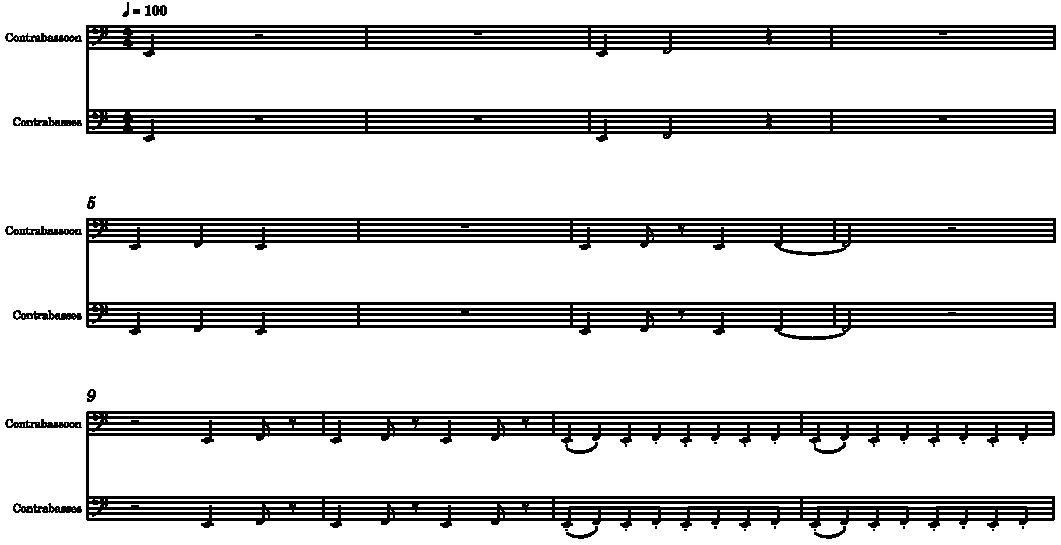
\includegraphics[width=1\linewidth]{img/president-jaws-intro.pdf}
    \caption{The opening 12 bars of \textit{Jaws}'s main title theme. The repeating minor second intervals shares similarities with Shire's ascending minor second motif.}
    \label{fig:president-jaws-intro}
\end{figure}

\subsubsection{C - Ascending Lydian Motif}

If the ascending minor seconds hint at the fractional progress made by the reporters, the ascending Lydian motif makes this a core aspect.
This is a simple, four-note motif that is repeated several times in each of its occurrences, with the exception of the film's final cue where it is only heard once.
It is therefore the motif that is heard the most, occurring in five cues, and the final motif that is heard in the entire score.
With the exception of this final cue, the motif's circularity points to the reporter's seemingly endless task; continuously ascending but never ultimately landing at a new destination.

The presence of the augmented fourth makes the motif function within the Lydian mode.
The Lydian mode as been desccribed as connoting generally optimistic feelings.
David Temperley and Daphne Tan explored this is a study wherein they played musical modes to participants to ascertain their emotional connotations.
They ultimately concluded that ``generally, happiness increases as scale-degrees are raised.”\autocites[][255]{temperley_emotional_2013}
Frank Lehman makes a similar argument in his thesis on tonalities in film music, citing the Lydian mode's ``victorious, childlike, and optimistic connotations."\autocites[][31]{lehman_reading_2012}
This motif, however, does not present these tonalities, and instead creates more of a sense of mystery and the unknown, appropriate to the film's themes of conspiracy and paranoia.

Janet Halfyard writes of the use of the tritone in horror scoring, an interval that is created through the augmented fourth in the Lydian mode and can be heard in this motif between the root C and F\sharp.
Halfyard's focus is on horror-comedies, and yet much of her analysis can be drawn upon for this particular motif.
She notes that each of the seven modes contain tritone intervals, but only the Lydian mode contains that interval in relation to the tonic.
The augmented fourth notwithstanding, the Lydian mode is otherwise fully tonally diatonic, thus allowing composers ``to be altogether more duplicitous in writing music that superficially sounds quite innocent but that conceals (and ultimately reveals) the devil."\autocites[][28]{halfyard_mischief_2010}
Such extreme revelations is of course hyperbolic with regards to the Watergate scandal.
However, the assertion that the Lydian mode can subtly hint at untoward practices remains useful in the context of \textit{President's Men}.
This augmented fourth can therefore be understood as representing the nefarious political action of Richard Nixon's administration, hiding in plain sight and easily overlooked among the socio-political landscape and otherwise diatonic tonality.

Another common trope in horror film scoring that is also evident in this motif in the use of repetition.
This has been discussed by Kevin Donnelly in his analysis of John Carpenter's \citetitle{carpenter_fog_1980} (1980).
He writes that ``repetitive music functions to induce instant tension as well as having a cumulative effect of disquiet or extreme anxiety."\autocites[][161]{donnelly_hearing_2010}
This assertion seems applicable in the case of this motif, with its highly repetitive nature, along with its somewhat unfamiliar Lydian melodic ascent, seeming to mirror the sense of paranoia that the film is dealing with.
The repetition also creates a soporific effect on the spectator, its repetitive, cyclical nature at times creating an ethereal and dreamlike quality.
This is often inspired by the instrumentation and the timbre of the piano or harp that performs it, which I will discuss further below.


\subsubsection{D - Hunting Fanfare}

This fanfare is only heard at one point in the film, following the first instance of the ascending minor second motif when Woodward is returning from one of his clandestine meetings with Deep Throat.
It is performed here on a French horn, and both the timbre and the film's depiction of an investigation harkens back to the ``most direct predecessor of the modern-day `French’ horn … the hunting horn.”\autocites[][22]{mckinney_forest_2020}
It thereby evokes images of ``the hunt” by drawing upon the historical connotations of the French horn.
This is further done by placing the fanfare in the horn’s upper register, a pitch that, as Raymond Monelle notes, ``old hunting calls … freely used."\autocites[][102]{monelle_horn_2001}
The hunt in this case appears to refer to the reporters’ investigation.
Yet it also adds an additional instance of foreshadowing, as we learn from a later meeting with Deep Throat that the reporters have become a target for the White House and that their lives are in danger (02:01:50).
Following this revelation, it is apparent that the reporters are now literally being hunted.
As I referenced above when discussing the minor second motif, there seems to be a sonic allusion to John Williams' main title from \textit{Jaws}.
Although this was somewhat subtle at first, this fanfare makes the connection far more explicit as we hear a similar French horn fanfare in Williams' cue (Figure \ref{fig:president-jaws-fanfare}).

\begin{figure}
    \centering
    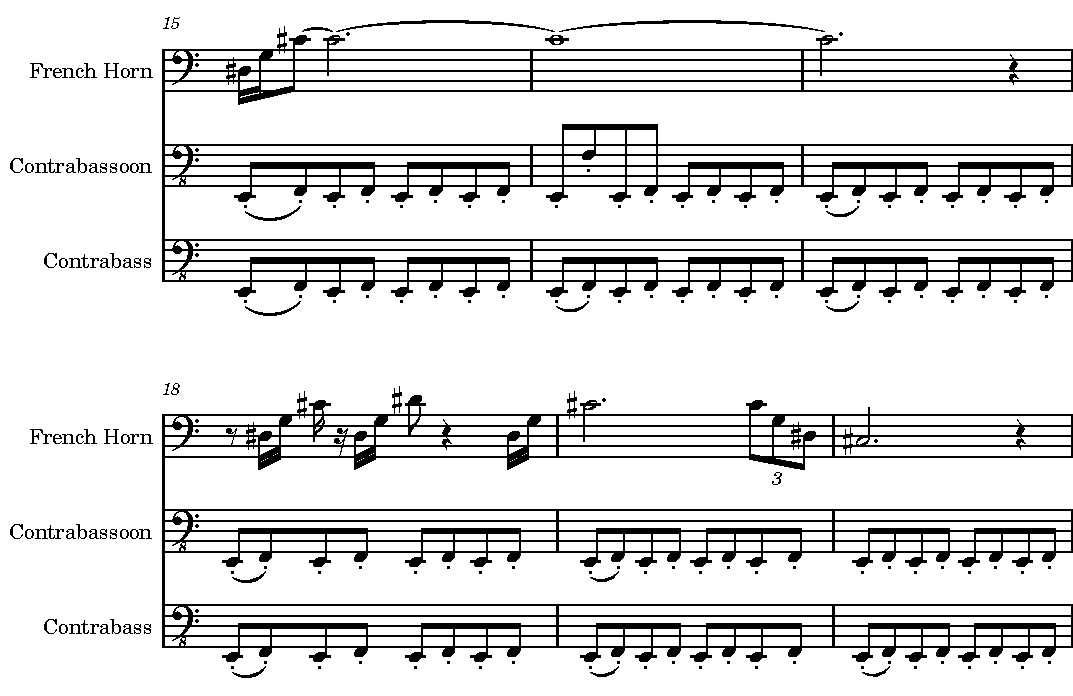
\includegraphics[width=1\linewidth]{img/president-jaws-fanfare.pdf}
    \caption{A reduction of John Williams' \textit{Jaws} theme. The ascending French horn motif seems an obvious influence for David Shire's ``To Deep Throat."}
    \label{fig:president-jaws-fanfare}
\end{figure}

Released less than a year before \textit{President’s Men}, and given its ubiquity and mass popularity, upon the release of \textit{President’s Men }in 1976 it would likely have been difficult to hear this cue without being reminded of \textit{Jaws}’ shark hunting its prey.
When considering each films’ use of French horn motifs, it is easy to draw a parallel between \textit{Jaws}’ shark, literally hunting its prey, and \textit{President’s Men}’s reporters, as they ``hunt” for their story.
Vincent Canby made this connection explicitly in his 1976 \textit{New York Times} review for \textit{President’s Men}, when he described it as ``the thinking man’s `Jaws.’"\autocites[][]{canby_presidents_1976}

\textit{President’s Men} subverts \textit{Jaws}’ narrative by turning the film's protagonists, and the spectators' avatars, into the ``hunters.”
Yet, while the reporters may be hunters in one sense, the musical allusion to \textit{Jaws} suggests that they, too, are being hunted.
In the same way that \textit{Jaws}’ theme alerted audiences to the presence of the shark, here the horn fanfare suggests that there is an unseen, malignant figure stalking Woodward.
It is never revealed whether Woodward is in fact being followed.
However, the aural reference to \textit{Jaws} can be inferred as a subtle allusion to a similarly antagonistic presence stalking him.
Both the reporters and the president’s men are thus simultaneously the shark and the beach-goers.

This allusion to \textit{Jaws} also reveals a link to notions of American identity.
This comes when focusing on Williams' French horn fanfare which seems to echo the trumpet fanfare from Aaron Copland's ``Fanfare for the Common Man."
Copland's ``Fanfare" was written in 1942, commissioned ``as a patriotic morale booster" to honour soldiers in World War II.\autocites[][5]{pollack_copland_2005}
It has subsequently become closely associated with a distinctly nationalist and pro-American ideology, despite Copland's desire to create a piece of music that transcended national boundaries.
``Fanfare" opens with what Stanley V. Kleppinger calls a ``triumphant exordium," an exuberant opening fanfare that became ``one of a handful of `Copland sounds' that have become intertwined with American identity."
A clear similarity can be found when comparing the triumphant exordium of ``Fanfare" with the more sinister fanfare heard in \textit{Jaws}.
With the knowledge that Copland was a major influence on Williams, this comparison feels justified and perhaps not accidental.\autocites[Emilio Audissino discusses the influence of Copland on Williams, claiming that ``Williams was also influenced by Copland's Americana dialect–pandiatonicism and quartel harmony–especially in his American themes."][139]{audissino_film_2021}
Williams has taken even more obvious influence from ``Fanfare" for his own cue for the 1996 Atlanta Olympics, ``Summon the Heroes."
Figure \ref{fig:president-jaws-copland} shows the fanfares heard in ``Fanfare for the Common Man", \textit{Jaws}, \textit{President's Men}, and, to evidence the influence of this specific Copland piece on Williams, ``Summon the Heroes."
For clarity and to aid my comparison, each of these cues have been transposed to open on middle C.

\begin{figure}
    \centering
    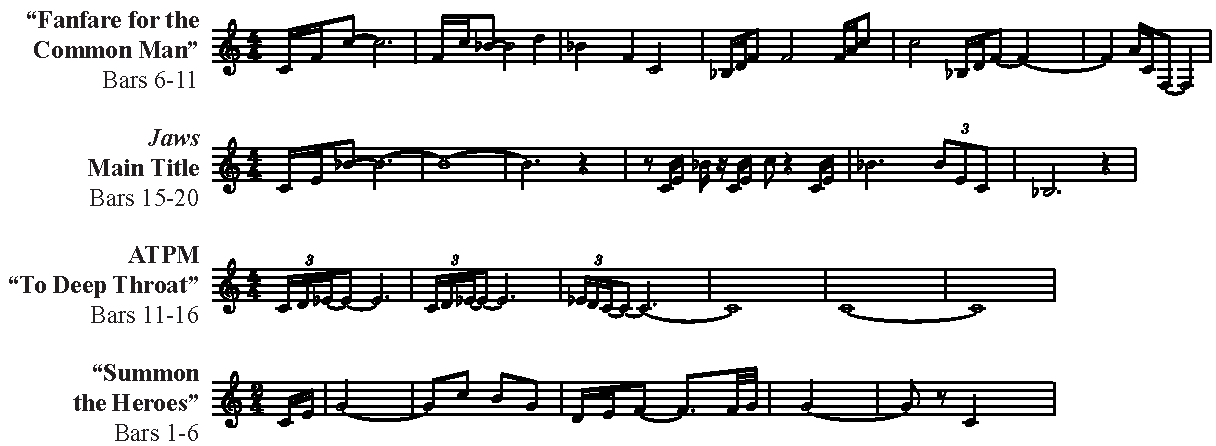
\includegraphics[width=1\linewidth]{img/president-jaws-copland.pdf}
    \caption{Brass fanfares heard in Aaron Copland's ``Fanfare for the Common Man," John Williams' main title for \textit{Jaws}, ``To Deep Throat" from \textit{All the President's Men}, and Williams' ``Summon the Heroes."}
    \label{fig:president-jaws-copland}
\end{figure}

Figure \ref{fig:president-jaws-copland-para} highlights similarities between Copland's and Williams' fanfares, with two phrases from Williams' score in particular containing what seem specific references to the earlier piece.
As column A shows, Copland's piece opens with an ascending perfect fourth followed by an ascending perfect fifth to the tonic.
Williams' on the other hand subverts the uplifting patriotism of Copland's fanfare by rising a major third and then a diminished sixth, creating a far more unsettling ambience.
Despite the differences in melodic contours, both fanfares share the exact same rhythm.

\begin{figure}
    \centering
    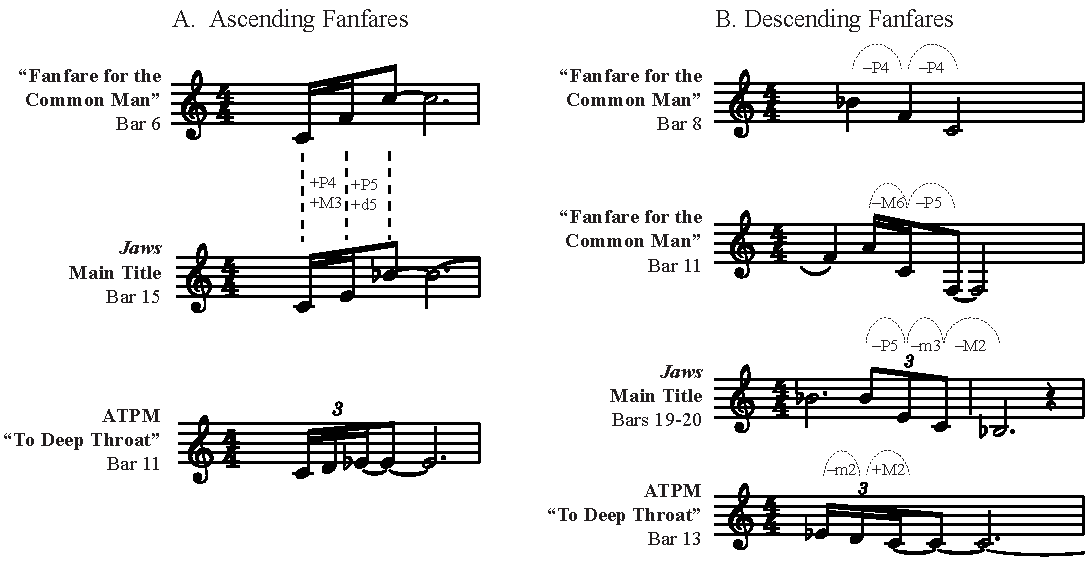
\includegraphics[width=1\linewidth]{img/president-jaws-copland-para.pdf}
    \caption{Phrases heard in the fanfares of Aaron Copland's ``Fanfare for the Common Man," John Williams' main title for \textit{Jaws}, and ``To Deep Throat" from \textit{All the President's Men}. Column A depicts the ascending fanfares. Column B depicts the responding descending fanfares that follow.}
    \label{fig:president-jaws-copland-para}\end{figure}


Another similarity is seen in both fanfares' descending motifs in column B.
Although the rhythms differ in each phrase, there is a similarity between Copland's and William's response to their own ascending fanfares, specifically in ``Fanfare's" bar 8 and \textit{Jaws}'s bar 19.
The slight difference in intervals, however, reflects \textit{Jaws}'s sinister interpolation of Copland's piece.

The significance of \textit{Jaws}'s citing of Copland's ``Fanfare" is evident when considering one of its core themes: the apparent crisis of masculinity in contemporary American society.
Michael Ryan and Douglas Kellner, for example, cite the film's shark as a ``sign of what goes wrong when the male sex is not fulfilling its duty of patriarchal leadership."\autocites[][60]{ryan_camera_1988}
The film focuses on three primary male characters as they hunt down the shark that is terrorising the coastal town of Amity: Brody, the police sheriff unable to protect his family and community or to assert his own physical presence; Quint, the brash and vulgar shark hunter; and Hooper, the younger, metropolitan academic.
While each figure represents a different iteration of masculine identity, the film's primary thematic clash is acted out between Quint and Hooper, the former representing an ``aggressive, hard masculinity," the former a contemporary, softer and more thoughtful masculinity. 
This was argued by Barry Monahan who considers the significance of characters' hands in portraying the theme of masculinity.
Monahan specifically cites one scene in which Quint denigrates Hooper for having ``city hands," an apparently feminine trait that betrays his lack of traditional American manhood.\autocites[][250]{monahan_hands_2022}
Their physical bodies thus become ``symbolic points of acting out their respective masculinities."\autocites[][251]{monahan_hands_2022}

\textit{Jaws} therefore can be read as a commentary on the downfall of traditional, Turneresque masculinity.
Williams' allusion to Copland's ``Fanfare" in turn becomes an ironic commentary on manhood in 1970s USA:
while Copland's piece celebrates the bravery and patriotic duty of servicemen in the Second World War, \textit{Jaws} addresses the lack of such commendable displays of masculinity.

\textit{All the President's Men} similarly reflects upon the failure of such patriarchal masculinities, specifically the nation's political leaders.
As I detailed in my introduction, the revelations that these leaders had failed to live up to the moral and legal standards many held them to, contributed to the ubiquitous sense of paranoia that had cumulated throughout the previous decade.
Since both films share this theme, Shire's referencing of Williams' score seems fully justified.\autocites[This connection is exacerbated in some analyses of \textit{Jaws} which draw a parallel between President Nixon and Amity's Major Vaughn, who insists on keeping the beaches open to maximise tourist revenue despite the evident threat posed by the shark. Peter Biskind, for example, notes that Vaughn ``repeatedly invokes `the public interest' as Nixon invoked `national security' to legitimate the various extravagances of his administration."][]{biskind_jaws_1975}

Both films ultimately see their protagonists succeed in their goals – explicitly shown in \textit{Jaws} as the shark is killed; and more subtly in \textit{President's Men} as a post-script details the president's downfall.
They differ, however, as \textit{President's Men} is less downcast in its portrayal of masculinity.
Its two reporter protagonists are never suggested as lacking in their patriarchal leadership capabilities.
Rather, the film celebrates their individualistic, dogged entrepreneurialism, and their willingness to exert their dominance over women in lesser positions of power, as I discussed in section  \ref{sec:president-themes}.
\textit{President's Men} is thus more optimistic about the rectitude of the American ideology, and so is more aligned with Turner's vision of American identity and the patriotic ideals of Copland's ``Fanfare."
Pakula himself seemed to make this explicit this when discussing the contrasting ideologies of his paranoid trilogy, explaining that ``\textit{Parallax View} represents my fear about what's happening in the world, and \textit{All the President's Men} represents my hope. Like most of us, I'm balanced between the two."\autocites[Pakula, quoted in][]{aquilina_all_2021}

%The implicit reference to Copland here instead seems to comment more on the general state of the American socio-political landscape on a more macro level.

By referencing \textit{Jaws}, Shire's fanfare implicitly evokes Copland's nationalism.\autocites[Although Copland's influence on Shire's compositional practices has been less documented than Williams', Juan Chattah notes that he was exposed to Copland's work from a young age and this ``had a profound effect on Shire, and triggered his interest in contemporary concert music."][2]{chattah_david_2015}
Figure \ref{fig:president-common} shows Copland's and Shire's fanfares side by side and highlights the intervallic differences, but also their rhythmic similarities.
As with figure \ref{fig:president-jaws-copland}, both motifs have been transposed to begin on middle C.
When seeing Copland's wide interval leaps contrasted with Shire's much smaller steps, we can see Shire's cue as a far more ominous and pessimistic.
Shire does not appear to strive for a similar sense of nationalistic pride as Copland does.
While \textit{Jaws} sharply critiques contemporary masculinity, \textit{President's Men} appears here more mournful for the state of the nation and patriarchal positions of power during the nation's ``post-traumatic" period.\autocites[][]{keathley_trapped_2004}
The more muted fanfare can be understood as more of a lament to the fading moral authority and reverence of the American identity than \textit{Jaws}'s ironic reference to American masculinity.

\begin{figure}
    \centering
    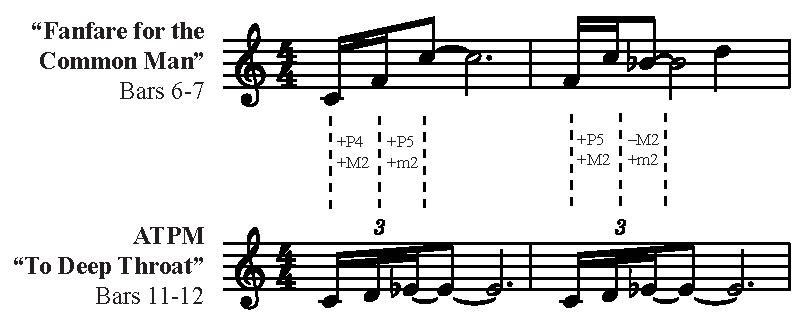
\includegraphics[width=1\linewidth]{img/president-common.pdf}
    \caption{The ascending fanfares of Copland's ``Fanfare for the Common Man" and David Shire's ``To Deep Throat."}
    \label{fig:president-common}
\end{figure}


\subsubsection{F - Alternating Perfect Fourths
}
While each of the previous motifs discussed thus far contain very small intervals or modal melodies which contribute to a tense and mysterious atmosphere, this motif introduces a much lighter tonality in contrast.
This motif is heard four times throughout the film, making it one of the most common motifs, and provides respite from the more sinister tonalities of earlier motifs.
Its series of alternating perfect fourths, followed by a minor sixth, remain fully diatonic and less troubling than earlier motifs.
This diatonicism, coupled with each phrase's whole tone ascent, creates an uplifting and more optimistic atmosphere.

Also contributing to this atmosphere is both versions of the motifs' intervals which are among the largest heard throughout the entire score.
The relevance of this to the film's emotional resonance is made evident with a consideration of Aalf Gabrielsson and Erik Lindström's meta-analysis of studies on musical structure and emotional affect, in which they note that ``large pitch variation may be associated with happiness, pleasantness, activity, or surprise; small pitch variation with disgust, anger, fear, or boredom."\autocites[][389]{gabrielsson_role_2010}
This understanding of musical expression reflects a more optimistic attitude to the reporters' progress, while the upward progression of each consecutive phrase further points to this.

Perhaps the most notable aspect of this motif is the repeated use of the perfect fourth intervals.
Returning to Neil Lerner, this interval has been understood as ``represent[ing] the vastness of nature," particularly in the works of Aaron Copland.\autocites[][503]{lerner_coplands_2001}
In Copland's music the celebration of nature can be extended to represent a celebration of America and Americanness.
Lerner here cites the opening to Copland's \textit{Appalachian Spring}, which opens with an A pedal and sees a series of consecutive ascending fourths which were intended to evoke images of America's open, rural landscape.
Prior to the introduction of these fourths, a clarinet performs an alternating motif, much like Shire's alternating motif here.
While Lerner's focus is on Copland's fourths, this clarinet motif contains alternating major thirds.
Despite this difference, however, Shire's motif echoes Copland's evocation of the American identity.
\begin{figure}
    \centering
    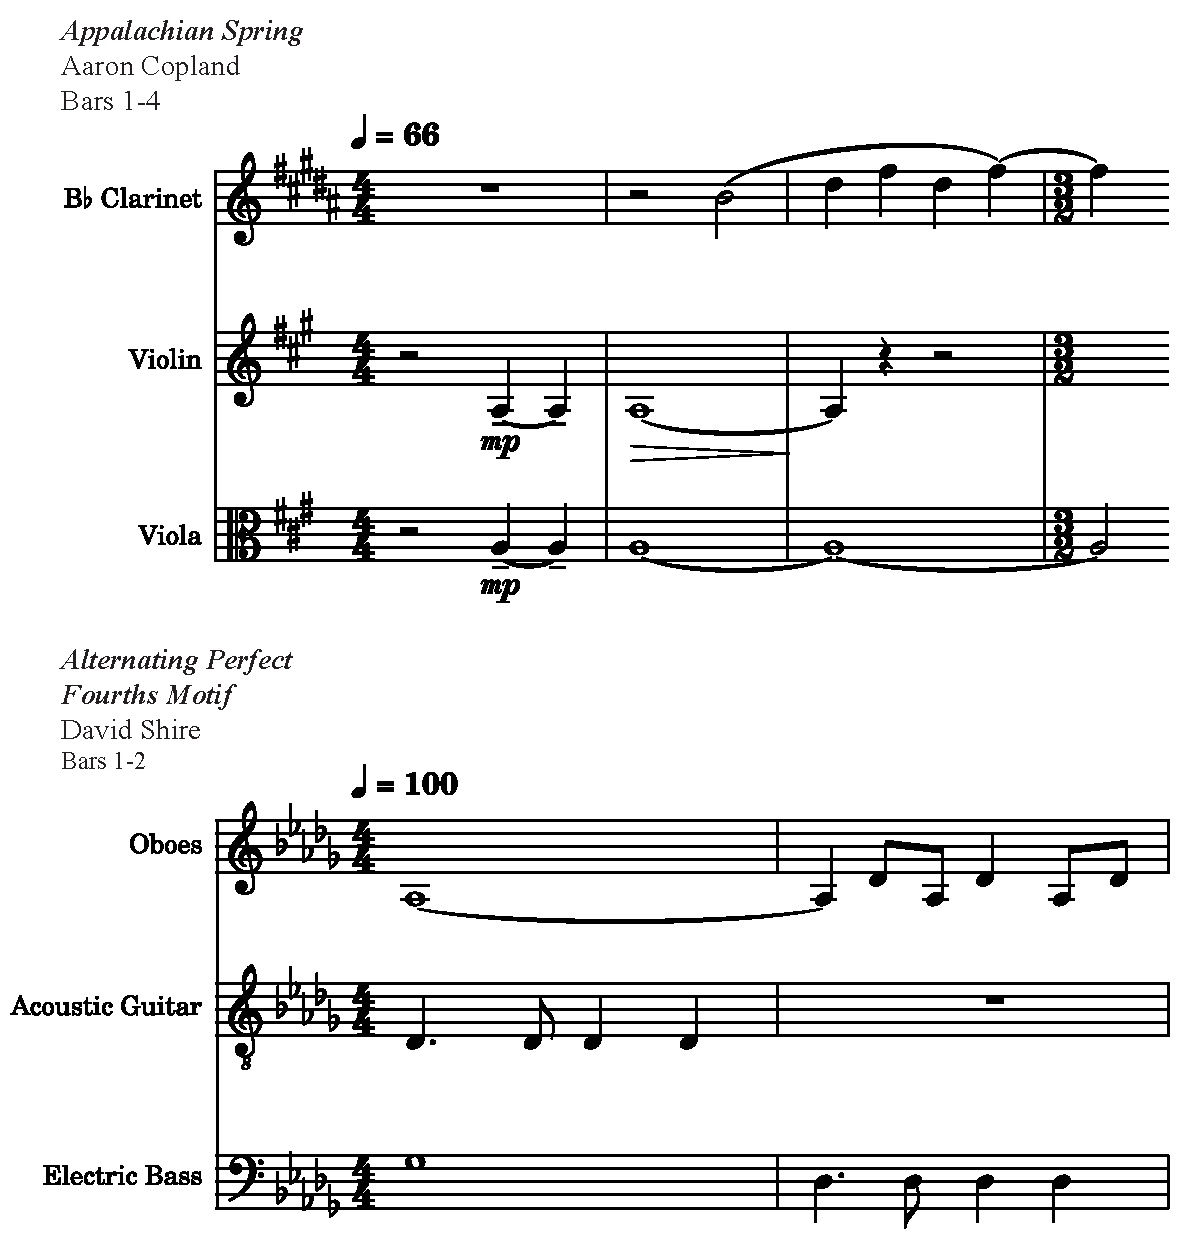
\includegraphics[width=1\linewidth]{img/president-fourths-appal.pdf}
    \caption{The opening bars of Aaron Copland's \textit{Appalachian Spring} and the first occurrence of David Shire's alternating perfect fourth motif from \textit{All the President's Men}. Both passages feature an alternating motif performed over a bass pedal.}
    \label{fig:president-fourths-appal}
\end{figure}

Figure \ref{fig:president-fourths-appal} shows this motif in the opening bars of \textit{Appalachian Spring}, alongside Shire's perfect fourths motif as it is first heard in the cue ``CREEP Sequence III."
As this figure demonstrates, both passages contain a simple, oscillating motif over a bass pedal.
Shire's motif thus appears to reference Copland's ``American idiom."\autocites[This phrase is taken from W. H. Mellers' discussion of ``American music," wherein he identifies several compositional practices that make up the ``American idiom." One of the key traits he identifies, and the most relevant for my discussion here is the ``feeling of vastness, enormous airiness and emptiness of space which probably derives from America's physical immensity and which is communicated through the music partly by the dominance of fourths and natural sevenths."][370-371]{mellers_american_1943}
The similarity between the two passages suggests an attempt by Shire to connote the American identity in a similar way to Copland.
As I have previously argued, \textit{President's Men} attempts to celebrate the idealised American identity at a time the greatness of such a figure was in doubt.
This use of a compositional practice that celebrates America in a largely sincere and uncritical manner can therefore be understood as Shire's allusion to this heroic American ideal.

An interpolation of the motif is heard at later stages of the film (see motif F2 in Figure \ref{fig:president-all-motifs}).
Although this is transcribed here as largely similar to the original version, it is performed at a slower tempo which more sustained notes in between the alternating intervals.
This less animated version of the motif suggests a steadier and less excitable atmosphere while retaining the Coplandesque tonality.

\subsubsection{G - Polyphonic Melodic Run
}
This motif introduces a new harmonic structure, as it is the first instance of multiple instruments performing polyphonic harmony.
It remains largely diatonic, with the exception of a single passing augmented second of an E\natural (bar 13, Figure \ref{fig:president-intertwining}).
Since this is only a brief passing note, it does not greatly disturb the harmonic consonance, which, coupled with the alternating fourths motif that this motif follows, provides a sense of comfort that other motifs do not.
Like the fourths motif, this mostly diatonic motif suggests a sense of progress in the film's narrative, and that the story is finally successfully being uncovered.

\begin{figure}
    \centering
    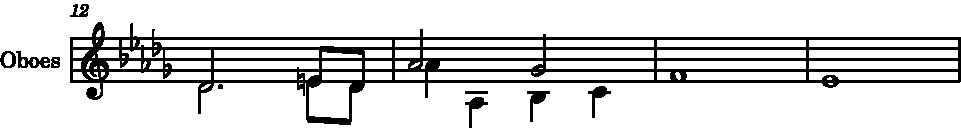
\includegraphics[width=1\linewidth]{img/president-intertwining.pdf}
    \caption{The polyphonic melodic motif presented as it is first heard in ``CREEP Sequence III."}
    \label{fig:president-intertwining}
\end{figure}

Additionally, the harmony between the two oboes reflects the improving working relationship between Woodward and Bernstein as they become more confident and comfortable working alongside each other.
This is similarly discussed in the reporters' book that the film is based upon, when they are writing about the sequence that this motif accompanies in the film:
\begin{quote}
gradually, Bernstein’s and Woodward’s mutual distrust and suspicions diminished. They realized the advantages of working together … The breadth of the story, the inherent risks and the need for caution all argued for at least two reporters working on it. … And, tentatively at first, they became friends.\autocites[While the book was written by the two reporters, it is written in the third person.][49-51]{woodward_all_1974}
\end{quote}
Nevertheless, the brief instance of non-diatonicism offers a subtle reminder of the conspiracy's complicatedness and sinister socio-political repercussions, and the tension that remained between the two reporters.





\subsubsection{H + I - Sustained Ascending Electric Piano + Frenzied Piano
}
The final cues to discuss do not appear in the same cue, but are heard closely together and contribute to a similar atmosphere of tension and paranoia.
Despite their emotional affect, they are largely oppositional in how they create this atmosphere.
Motifs H1 and H2, for example, are sustained drones that have a similar effect as the repeated motifs discussed above, and that Donnelly described as capable of evoking ``disquiet or extreme anxiety."\autocites[][161]{donnelly_hearing_2010}

The Frenzied Piano, on the other hand, is far more active and more obviously distressing with its high register and rapid movements.
These elements, and the ethereal timbre of the electric piano, align it with some contemporary horror scoring such as Carpenter's \textit{The Fog} that Donnelly discusses, as well as Mike Oldfield's ``Tubular Bells," heard in \citetitle{friedkin_exorcist_1973} (William Friedkin, 1973).
Figure \ref{fig:president-horror-synth}, for example, showcases the title theme from \textit{The Fog} and the opening motif from ``Tubular Bells," which was used as \textit{The Exorcist}'s title theme.
Each of these motifs are built from repeated arpeggios performed by synthesizers and organs which create other-worldly, dream-like timbres.\autocites[On``Tubular Bells," Mike Oldfield utilised pianos, and multiple reed and electronic organs. As Donnelly notes, there is no official record of which specific synthesizer Carpenter used on his score for \textit{The Fog}. Donnelly surmises that it was likely a Moog Series 3.][159-160]{donnelly_hearing_2010}

\begin{figure}
    \centering
    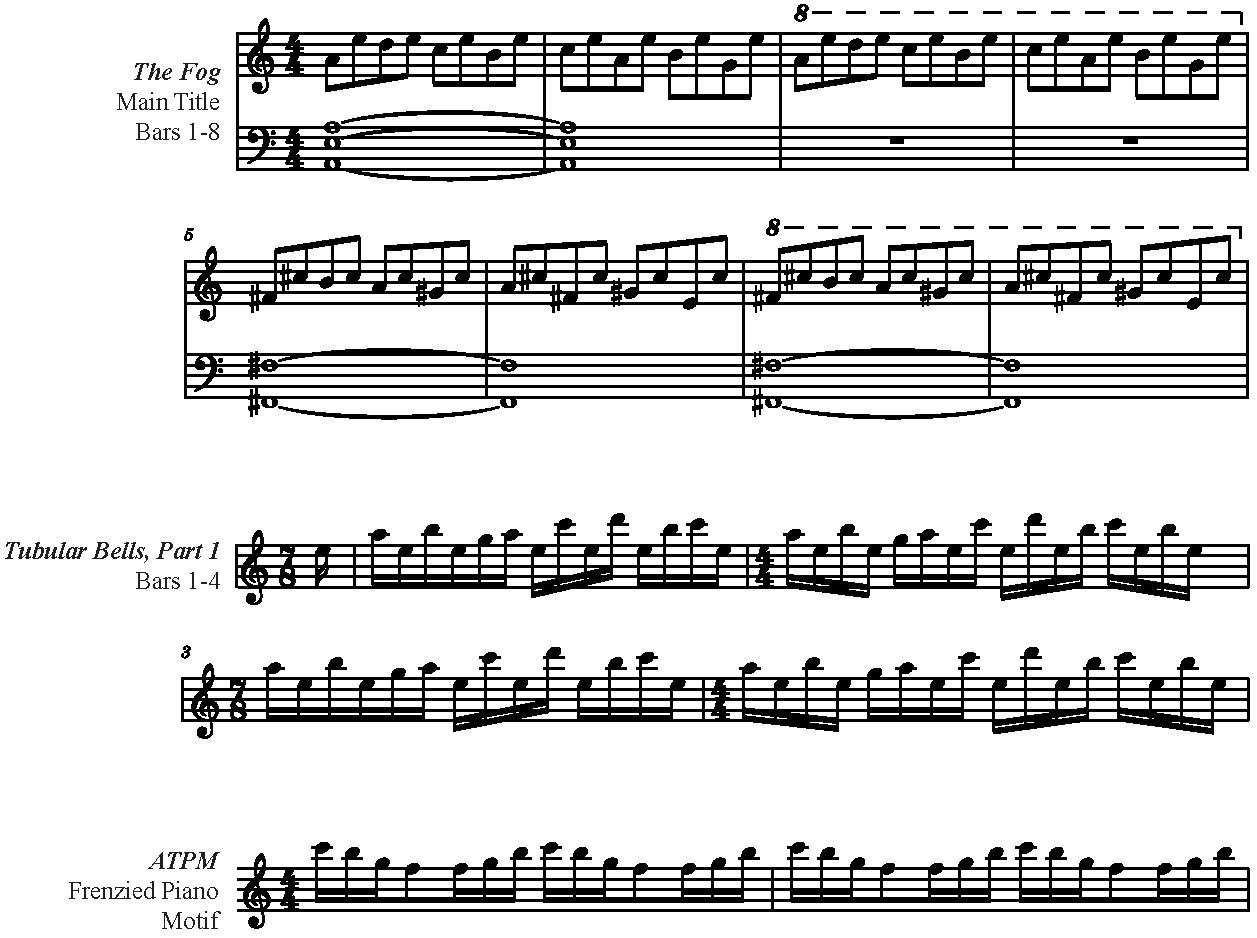
\includegraphics[width=1\linewidth]{img/president-horror-synth.pdf}
    \caption{The main title from John Carpenter's \textit{The Fog}, Mike Oldfield's ``Tubular Bells" heard in \textit{The Exorcist}, and David Shire's ``Frenzied" motif. All three motifs contain repeated arpeggios performed on ethereal keyboard instrumentation which contributes to a sinister, uneasy atmosphere.}
    \label{fig:president-horror-synth}
\end{figure}
Of course, \textit{The Fog} was released after \textit{President's Men}, but the horror that repeated arpeggios and electronic timbres evoke nevertheless remain.
Shire's motif here thus fits within a lineage of contemporary horror scoring, and is used reflect the sinister and uncomfortable atmosphere that was prevalent throughout this period.

This motif also reflects Shire's earlier score for \textit{The Taking of Pelham 123}.
As I noted above, Shire took inspiration for this score from Alfred Schoenberg's twelve-tone technique, which he combined with jazz to create a ``bewitching, funky, horn-heavy soundtrack that defied the tonal tradition of classical Hollywood film scoring."\autocites[][30]{chattah_david_2015}
Shire claimed that his intention for this score was to compose a ``New York jazz-oriented, hard-edged" score, appropriate for an action film set in the chaotic, urban milieu of 1970s New York.\autocites[][30]{chattah_david_2015}
Although \textit{President's Men}'s score does not aspire to a similar objective, brief elements can be heard in this motif.
Specifically, in a rapid melodic run heard in \textit{Pelham}'s main theme.
Figure \ref{fig:president-pelham} shows this motif, along with a brass melody that shares rhythmic and some melodic traits.
\textit{Pelham}'s motif here was composed with the aid of a twelve-tone matrix, which imbues it with a strong sense of disorder and non-diatonicism, whereas \textit{President Men}'s motif is less chaotic and more diatonic.
Despite their myriad differences, Shire's apparent reference to his earlier cue imbues this motif with a similar allusion to the urban chaos.
However, instead of reflecting the specificities of New York during this period, this motif reflects the chaos that was supposedly rampant throughout the country on a more macro level, as the nation collectively underwent its post-traumatic period.

\begin{figure}
    \centering
    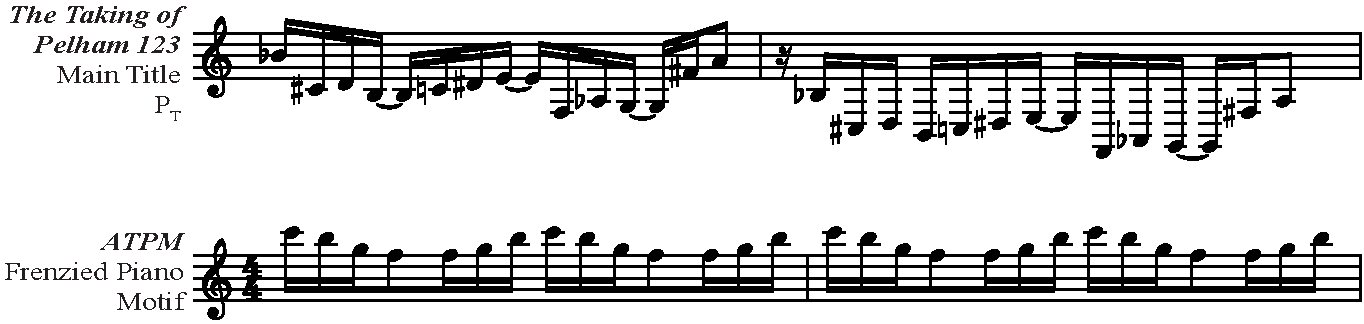
\includegraphics[width=1\linewidth]{img/president-pelham.pdf}
    \caption{A brass motif from David Shire's score for \textit{The Taking of Pelham 123}. Note that the use of both flats and sharps in the \textit{Pelham} motif reflects Shire's use of the twelve-tone technique. This motif is cited as $P_T$ following the twelve-tone matrix and transcription found in Juan Chattah's brief analysis of this theme.\autocites[][31-32]{chattah_david_2015} This melody is contrasted with Shire's frenzied piano motif from \textit{President's Men}, which follows a similar rhythmic structure.}
    \label{fig:president-pelham}
\end{figure}

Having discussed the above motifs in some detail, I will now move on to more specific analyses of cues to explore how these motifs are used throughout the film.

\subsection{Cues}

\subsubsection{Library of Congress}

The first instance of extradiegetic music occurs as Woodward and Bernstein visit the Library of Congress to gain information on books checked out by members of Nixon’s administration.
This cue is titled ``Library of Congress” (00:28:30).\autocite[I have taken the names of these cues from the soundtrack album released in 2007. Although the scores heard on this release are not exactly as they appear in the film, for ease of reference I will continue to refer to them as they relate to the soundtrack album.][]{film_score_monthly_film_nodate}
While they read through these documents, the camera peers down at them from above and pulls away toward the ceiling.
\begin{figure}
    \centering
    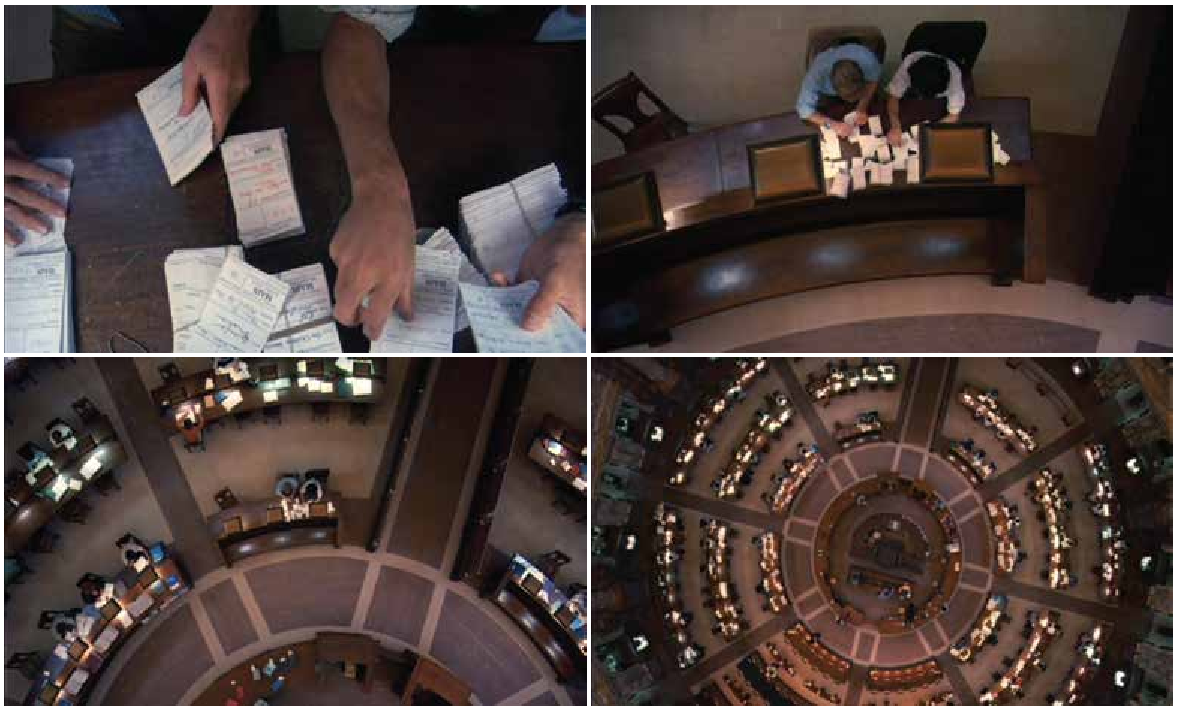
\includegraphics[width=1\linewidth]{img/president-library-dissolve.pdf}
    \caption{Woodward and Bernstein in the Library of Congress. The camera floats above them, dissolving several times as it gets higher (00:28:30)}
    \label{fig:president-library-dissolve}
\end{figure}
The shot dissolves several times as the camera continues to rise above the reporters, making them appear tiny within the grand setting (Figure \ref{fig:president-library-dissolve}).
The dissolves make the spectator quickly lose track of the reporters as, for the first time, we realise the magnitude of their task: two reporters researching a massive and complex governmental operation, the scale of which they do not yet realise.

This is the first time that Pakula directly employs more ``cinematic" camera movements.
Whereas prior to this sequence, the camera had generally remained static or tracked horizontally along with the characters, always generally remaining at eye level, here the camera floats above the reporters as if providing the perspective of some omniscient spectator.
The formalist perspective disrupts the docudrama aesthetic that had been established throughout the film to this point.
This first instance of scoring also acts to disrupt the relative realism of earlier sequences.
The seeming ``impossibility of their huge task,” as Terry Christensen described it, is further hinted at by the repetitive and soporific score which begins as the camera begins to pull away from them.\autocites[][133]{christensen_reel_1987}

The cue opens with two sustained bass notes from an electric bass guitar before it develops into the rhythmic heartbeat motif.
This motif provides insight into the reporters' subjectivities; the spectator experience their pulsating heartbeats as they search through the archives.
The bass's unwavering pitch also hints at the reporters' seemingly unending task, while its unsteady rhythm, with notes often occurring of the offbeat, denies the spectator a solid grounding.
This syncopation contributes to the film's generally discomforting atmosphere by mirroring the paranoia and tension of the protagonists and the nation.

The score subsequently expands with the gradual addition of a French horn performing the minor second motif, and a piano which introduces the Lydian motif (Figure \ref{fig:president-library-cue}).
These two non-diatonic motifs disrupt the presumed key of E\flat.
The dissonance these motifs create is at first only heard through passing notes, as in bar 7 of Figure \ref{fig:president-library-cue}.

\begin{figure}
    \centering
    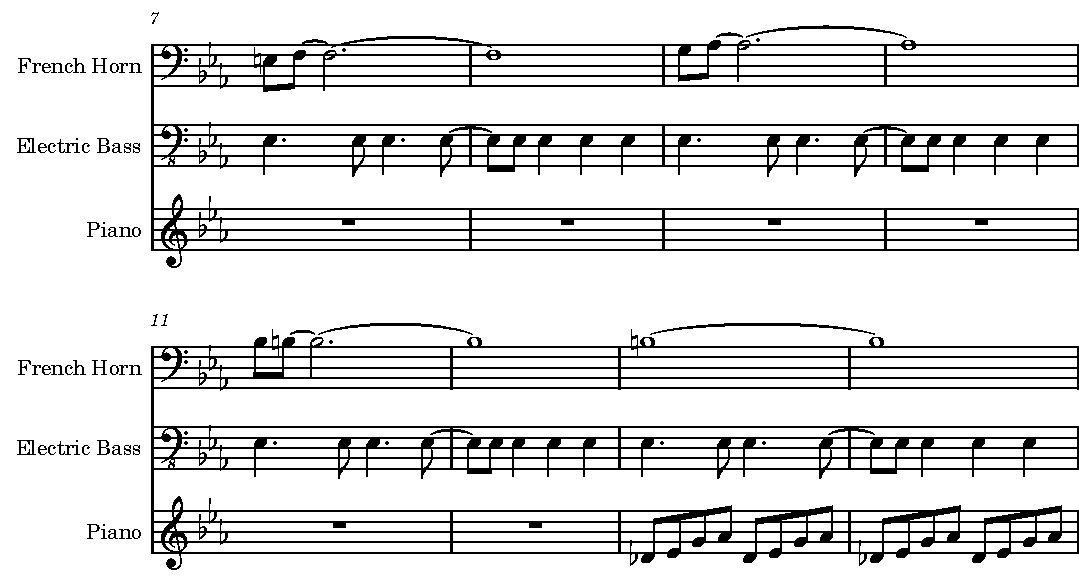
\includegraphics[width=0.75\linewidth]{img/president-library-cue.pdf}
    \caption{``Library of Congress." After several bars of the heartbeat bass pedal, the ascending minor second and Lydian motifs are introduced.}
    \label{fig:president-library-cue}
\end{figure}
However, bar eleven sees the horns ascending from B\flat to B\natural, the augmented fifth of the diatonic scale.
The augmented fifth of B\natural here can also be understood as C\flat, the flattened sixth of E\flat.
This interval between the root and flattened sixth is therefore suggestive of the Phrygian, Aeolian, and Locrian modes, each of which have sinister and ominous connotations.
This clash remains for the remainder of the cue, creating a continuous dissonance and denying any resolution or sense of relief.
While this dissonance is sustained, the lack of resolution is exacerbated with the introduction of the Lydian piano motif which rises without ever reaching its climax.

The repetition of the piano and the bass line, in addition to the dreamlike camera dissolves, have a hypnotic effect, which seems to allude to the tediousness of the investigation.
The small intervals in this sequence also reflect this by signifying the reporters' minimal progress, while its quietly ominous tone heightens the unsettling atmosphere that was fundamental to paranoid thrillers.
The piano's repetition can similarly be understood as representing the circularity and labyrinthine nature of the conspiracy the reporters are working to uncover.
The visuals also reflect it as the spectator loses sight of the reporters amid the vastness of the library.
And yet, the steady, unwavering bass pedal and piano melody also reflect the reporters' steadfast determination to continue their investigation regardless of any roadblocks.
It therefore highlights their self-sufficiency and resilience as motivated and driven heroes.

If understanding this cue as subtly acknowledging Woodward and Bernstein's capitalistic doggedness, it seems as though this sequence transfigures them as the mythical American heroes.
Noted above, this is complicated by the fact that the reporters are real people.
This sequence, however, sees them treated more like \textit{fictional} figures, as the extradiegetic score and the camera's artistic movement subverts the film's previously ``realist" aesthetic.
By employing more formalist techniques here, the reporters' mythic status is highlighted and their position as traditional film heroes and their representation of Turner's idealised American identity is foregrounded.


% \textcolor{red}{the small steps of the horns and piano reflects the little progress of W and B.
% What mode is the piano in? D Flat Lydian
% How does this pertain to Turner? By adding music here, it becomes more of a "film" and the reporters become more like "characters". Does this have an impact on how heroic they are? Can I make the claim that prioritising the fictionality and drama in this sequence, they are becoming more aligned with the traditional heroes?
% They are being self-sufficient and aggressive workers/capitalists. Can I argue this the point above about the small steps suggests this? the repetition of the piano reflects the little progress they're making AND their resilience! (this is a good one, something here!)}

This sequence ends with a cut to outside of the library.
We learn here that the reporters were unable to uncover anything to aid their investigation, and they are convinced that the evidence they were searching for has been tampered with.
``Library of Congress" can be understood as a signifier of the organisation the reporters are trying to discover.
Despite the reporters' relative naivety of the size of the operation at this point, the cue provides subtly suggestions that what they are researching will prove to be a sinister and dangerous conspiracy.
Further foreshadowing is evident through the repeated use of dissonance and lack of resolution, which alludes to Woodward and Bernstein's inconclusive research.


\subsubsection{To Deep Throat}

A new cue is heard shortly after this scene and is heard in a similarly formalist sequence.
This cue, entitled ``To Deep Throat,” is introduced as Woodward discovers a message wrapped in his newspaper (00:33:11).
The cue begins as soon as the note is shown to the camera and continues through the following travelling sequence.
On his way to meet Deep Throat in a car park, Woodward changes taxis multiple times and is constantly looking over his shoulder, demonstrating the extreme measures they are taking to remain secretive.
The sequence also acts to heighten the sense of paranoia since the spectator is made to believe that Woodward is likely being followed.

This cue largely follows the same structure and instrumentation as ``Library of Congress," with the Heartbeat Bass and French horn's Ascending Minor Second motif.
Whereas the horn concluded with the flattened sixth in ``Library of Congress," here it goes on to perform the Hunting Fanfare motif (Figure \ref{fig:president-deep-fanfare}).
Despite the change in melodic structure, the first two phrases of this motif end with a sustained flattened sixth, again creating a dissonant pedal between the bass and the horns.
The horn's descending run, however, lands on A\flat, creating a perfect fourth above the root note in the bass line.
The consonance here provides a very slight sense of comfort,.
When considering my argument above that the Hunting Fanfare is a lament to the fading dominance of the Turneresque patriarch, this consonance provides a subtle nod to the comfort that that figure should provide.


\begin{figure}
    \centering
    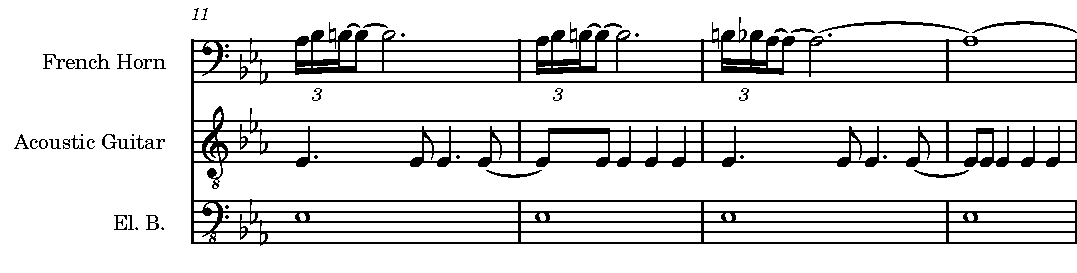
\includegraphics[width=1\linewidth]{img/president-deep-fanfare.pdf}
    \caption{``To Deep Throat." The French horns perform ascending and descending triplet motifs.}
    \label{fig:president-deep-fanfare}
\end{figure}
The ascending Lydian piano motif also returns in this cue, although it is not played as continuously as the previous cue.
Instead, it is played three times before stopping and returning again on the third beat of the bar, allowing the horn's motif to take prominence.
The infrequency of the piano's presence creates an even far unsettling atmosphere than when it was heard consistently.
For while its repetitive use in ``Library of Congress" created discomfort through its lack of resolution, in ``To Deep Throat" its more sporadic use denies the spectator a consistent sense of grounding.
The tension of the scene, as we see Woodward attempting to evade potential hunters, is therefore heightened.

This is perhaps the first time in the film where the sense of paranoia that was supposedly ``infecting the nation" becomes manifest:\autocites[][416]{perlstein_invisible_2014}
Woodward seems convinced he is being followed and takes many careful steps to lose his pursuers, while the score creates a tense and uneasy atmosphere.
The cue makes such an idea seem perfectly acceptable, and the subtle allusion to \textit{Jaws}' main title in the Hunting Fanfare seems to make a direct reference to those ``hunting" Woodward.
Through the constant surveillance that Woodward is under – alluded to by his covert actions in travelling to Deep Throat and the Hunting Fanfare – the threat to his personal safety and his individualist freedoms are foregrounded.


\subsubsection{Unifax}

The next cue, ``Unifax," is played as the spectator is shown a close-up of a newspaper heading from a rival newspaper, \textit{The New York Times}: ``Calls to G.O.P. Unit Linked To Raid on the Democrats” (00:39:17).
Woodward and Bernstein vent their frustration with missing out on this scoop. Despite their frustration, the cue presents a soft and light tonality through the presence of a harp and a contrabassoon, performing the Lydian and the Ascending Minor Second motifs, respectively (Figure \ref{fig:president-unifax}).

The smooth, lilting sound of the harp presents a less harsh and more soothing soundworld than that created by the earlier use of the piano.
The use of B Lydian, nevertheless, retains its ambiguity which is furthered by the harp’s ethereal and otherworldly timbre.

\begin{figure}
    \centering
    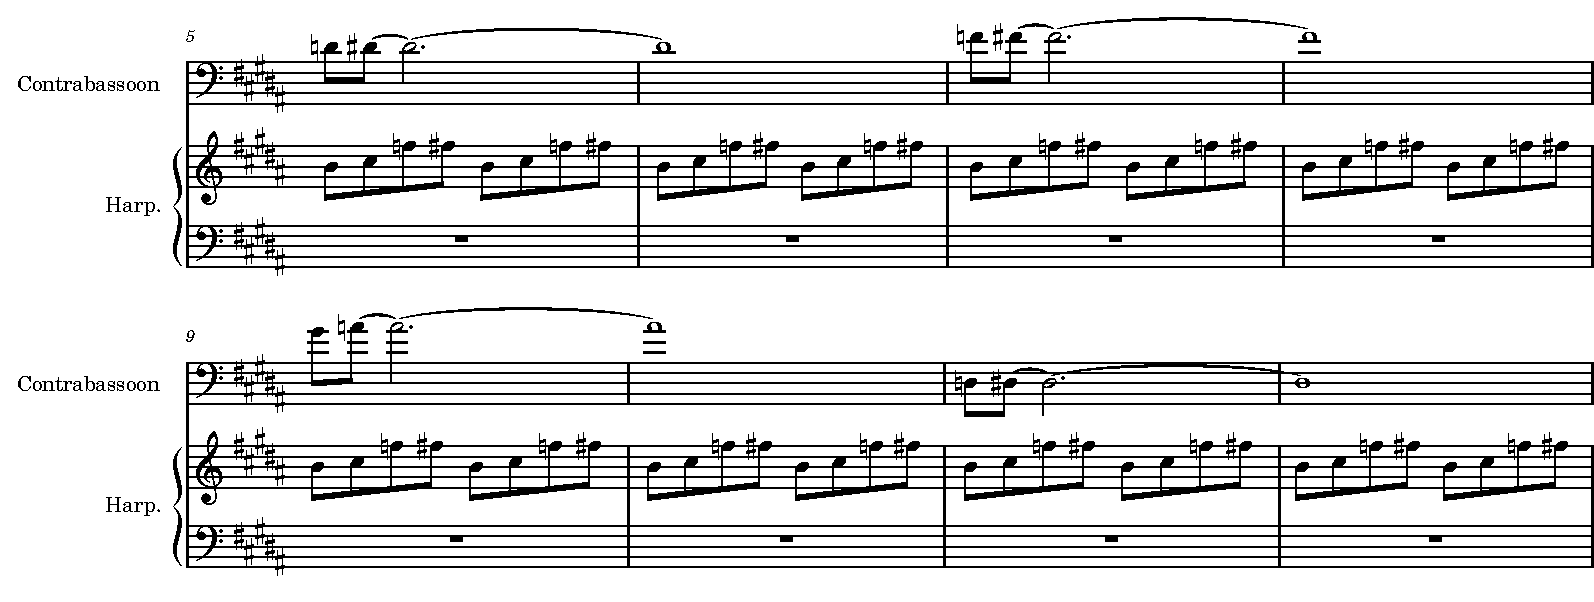
\includegraphics[width=1\linewidth]{img/president-unifax.pdf}
    \caption{The previously heard ascending Lydian motif and minor second motifs are heard in ``Unifax," played by a harp and contrabasson, respectively.}
    \label{fig:president-unifax}
\end{figure}
Similar to the harp, the smooth timbral qualities of the contrabassoon stand in stark contrast to the French horns which provided a far more aggressive sound quality.
The contrabassoon creates a gentler tonality, and yet its quivering vibrato suggests a semblance of uncertainty, denying the spectator complete comfort.
The instrumentation subsequently presents a sonic juxtaposition to their motifs: the warm sonic qualities of the harp and contrabassoon are contrasted with the tonal ambiguity and dissonance of their respective motifs, further contributing to the unsettling ethereality. 

While the motifs are recycled from earlier cues – albeit in a different key – the reordering of their introduction and the shift in instrumentation points to confusion regarding the constantly shifting nature of the Watergate story.
For as soon as the reporters think they understand it, they realise they had it all in the wrong order.
This is further exacerbated by the repetition of the contrabassoon’s Minor Second motifs.

In previous cues, this motif was played three times and ends at its highest pitch.
However, in ``Unifax” the contrabassoon plays the motif three times, before ending the cue a whole octave lower than its original pitch (see bar 11 in Figure \ref{fig:president-unifax}).
Upon lowering its register an octave, the contrabassoon repeats the first ascending pattern in this motif, D-D\sharp.
Whereas the ascending notes of this motif suggest forward progression, this return to the lower register suggests a backwards step in the reporters’ investigation as they are beaten to a key breakthrough in the case by reporters at \textit{The New York Times}.

This cue’s tonal qualities, as I mentioned above, appear in contrast to the emotion shown by the reporters when they see their competitors' article.
While in “Library of Congress” I suggested that the score was representing their subjective perspectives, the music here does not align with their emotional state.
This raises the issue of whose point of the view the non-diegetic cues are representing, what Gérard Genette terms ``focalisation."
Focalisation determines from whose perspective a story is told, and can be internal – wherein a story is depicted as from a particular character’s consciousness – or external  – when the ``hero performs in front of us without our ever being allowed to know his thoughts or feelings."\autocites[][190]{genette_narrative_1980}

External focalisation is most applicable here, particularly when following its definition as laid out by James Buhler: 
``with external focalisation, the narration allows us to read characters’ faces, hear their voices, and see their actions to be sure, but we must draw inferences about psychology from outside, from observation.”\autocites[][177]{buhler_theories_2018}
Given that the film is told largely from the reporter’s point of view, Buhler’s definition is apt; we witness their discovery of information and their responses to the narrative events, but are not given insight into their emotional response.
More pertinent to my purposes, we do not \textit{hear} their emotional response.
In the case of ``Unifax," the soundtrack actively seems to contradict their subjectivities.
Rather than hearing a cue with abrasive, brass timbres that may be more fitting to the reporters’ emotional states, we hear two instruments with warm, soothing tonalities.
The music can again therefore be understood as representing the clarification of information as the truth is slowly revealed, with the more pleasing timbres suggesting a better understanding of the state of affairs.
Yet, despite this breakthrough in the case, the labyrinthine nature of the conspiracy remains, as represented by the tonal ambiguity and dissonance within the cue.


\subsubsection{CREEP Sequence Suite: I}

After a roughly 20-minute stretch without any non-diegetic scoring, the largest musical cue is heard.
This is a collection of three shorter cues that I dub the ``CREEP Suite," and is arguably the centrepiece of the film's soundtrack.
With little cinematic flourishes and no non-diegetic additions, this stretch of the film sees the reporters ... \textcolor{red}{WHAT HAPPENS IN THIS STRETCH?}
A montage sequence of Woodward and Bernstein visiting CREEP employees at their homes, accompanied by ``CREEP Sequence I" restates the film's more ``cinematic" aesthetic (01:01:34).

``CREEP Sequence I" opens with the Lydian motif played on a harp and an electric bass performing the Heartbeat motif on B\flat.
The cue is soon expanded with a French horn playing the Ascending Minor Second motif, and, for the first time, an acoustic guitar finger picking a B\flat major arpeggio with added major sixth passing notes.

The return of the French horn presents yet another shift in tonality.
Whereas the timbre of the vibrato contrabassoon of ``Unifax" created a soothing, if uncertain, sonic texture, the intensity and abrasiveness of the French horn suggests far more certainty and determination.
This is visually depicted by the reporters' persistence in trying to interview witness, despite repeatedly having the doors closed in their faces.
The horn also deviates from the previous occurrences of this motif, ending each motif with sustained notes rather than the third ascending phrase (see bars 7-10 and 15-18 in Figure \ref{fig:president-creep-I}).

The second instance of these sustained notes in bars 15-18 of Figure \ref{fig:president-creep-I} sees the horn ascends from the A\flat to C and descend to F, outlining a F minor triad in first inversion.
The suggestion of the minor subdominant here, played over the guitar's repeated B\flat major sixth, reinforces the tonal ambiguity that has been a constant through the score to this point.
\begin{figure}
    \centering
    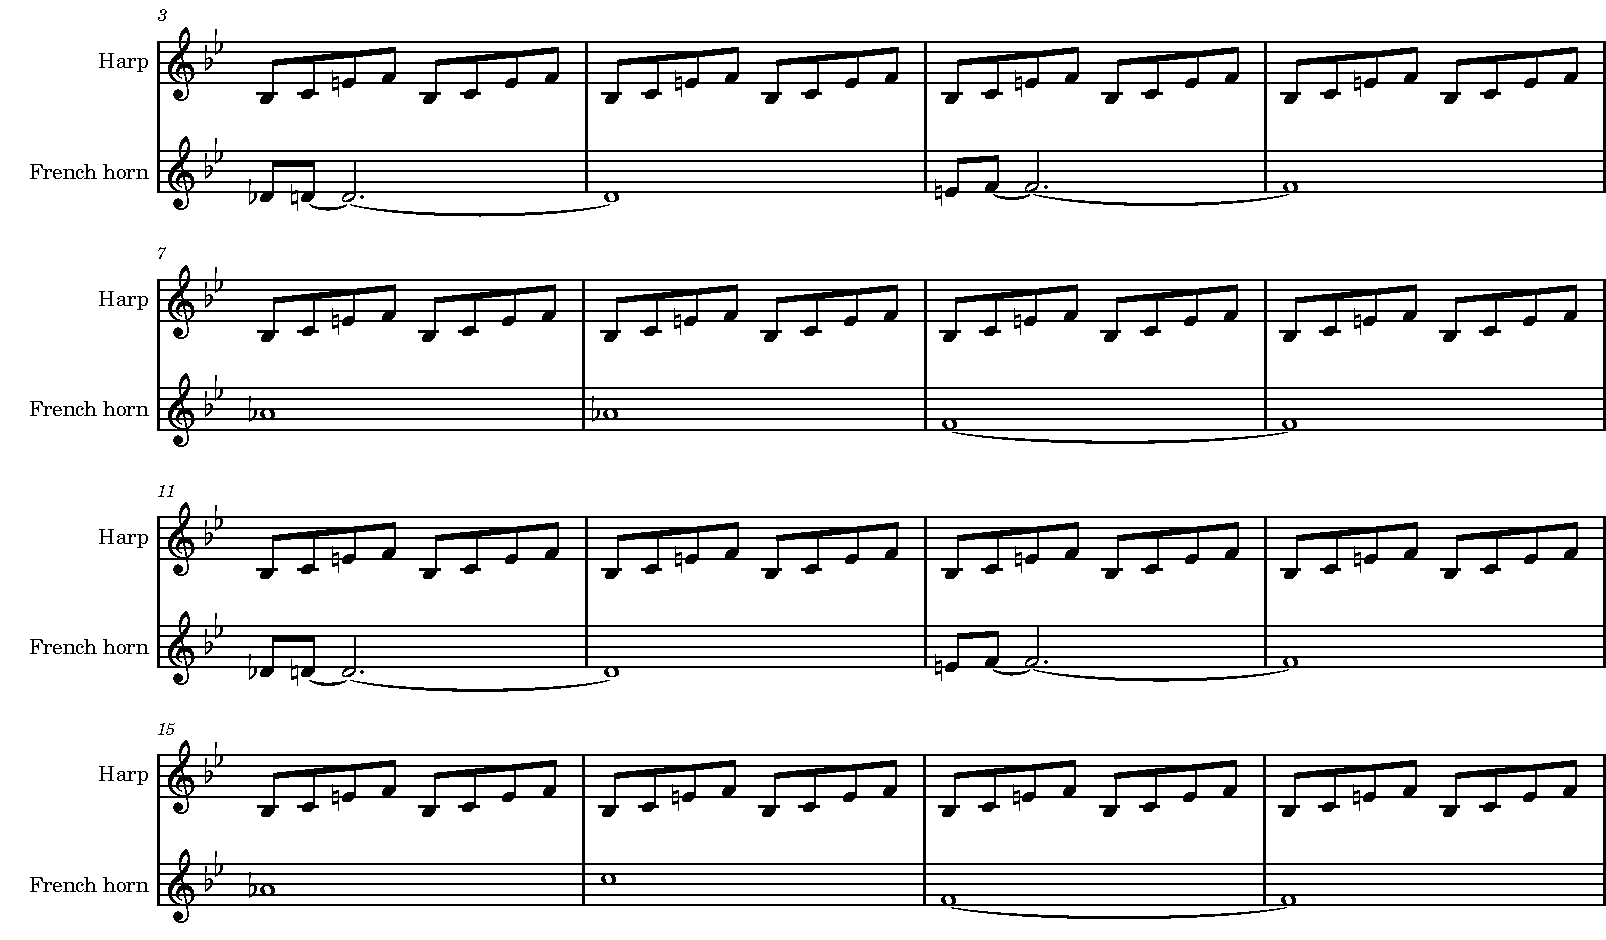
\includegraphics[width=1\linewidth]{img/president-creep-I.pdf}
    \caption{A reduction of the first cue heard in the CREEP Suite. In bars 7-10 and 15-18, the French horn motif deviates from the previously heard versions of the Ascending Minor Second motif by sustaining notes rather than the final ascending phrases.}
    \label{fig:president-creep-I}
\end{figure}
While the horn therefore varies its performance, the rest of the motifs are repeated with no variation.
The harp, acoustic guitar and bass guitar therefore provide a sense of stability, despite the discomfort that constant repetition can evoke.
This stability masks the brief instances of dissonance created by the passing non-diatonic notes.
As such, the instability and insecurity of this post-traumatic period is only subtly alluded to, and the cue therefore hints at the relative obscurity of the conspiracy hiding in plain sight.


\subsubsection{CREEP Sequence Suite: III}

The next cue in the CREEP Suite introduces a substantial change in tonality.\footnote{Although it is the second cue heard in the CREEP Suite, I cite this cue as III following the naming convention on the soundtrack album.}
Just as in the previous sequence, this cue accompanies a montage of the reporters knocking on doors to question witnesses (01:05:09).
It opens with the restatement of the Heartbeat motif which alternates between an electric bass and acoustic guitar.
The acoustic guitar's higher register provides a much lighter contrast to the lower, darker bass tone, and therefore creates a noticeably less ominous atmosphere.
The sense of foreboding remains, however, with the intermittent bass guitar's performance of the motif, 

Similar respite from the more sinister tones of earlier cues is provided in the light, airy timbres of oboes which are heard for the first time in this motif, performing the Alternating Fourths motif (Figure \ref{fig:president-creep-3}).
As I detailed above, this motif contains much larger intervals than those heard thus far, which, following Gabrielsson and Lindström, provides a comparatively optimistic tonality.
This understanding of musical expression reflects the reporters' belief that they are finally beginning to make significant progress in their investigation. 
Furthermore, the repeated fourth interval can be understood as representative of a celebratory Coplandesque evocation of the American identity.
This cue is heard as the reporters continue their investigation, persisting in their task regardless of the obstacles they encounter.
We therefore see the reporters here as the individualist, self-sufficient American ideal, thus are suitably accompanied by a compositional practice that Copland helped to ensure reflected the USA's praiseworthy character .
\begin{figure}
    \centering
    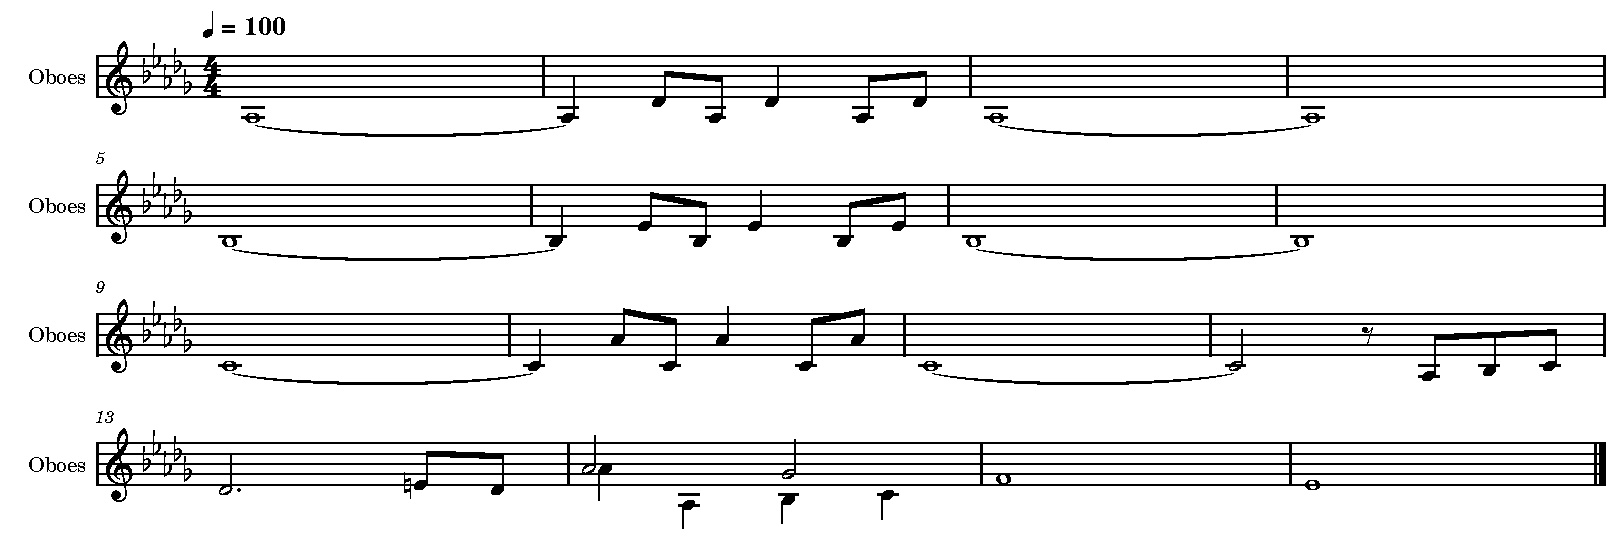
\includegraphics[width=1\linewidth]{img/president-creep-3.pdf}
    \caption{Oboes in ``CREEP Sequence III" introduce a new, consonant melody, before a harmonising run in bar 14.}
    \label{fig:president-creep-3}
\end{figure}
The oboes follow the Perfect Fourths motif with the Polyphonic Melodic Run, highlighting the interconnectedness of the two reporters.
This understanding leads us to appreciate each oboe as representative of each reporter, functioning independently and individualistically, while complementing each other and reaching a consonant, unified conclusion at E\flat.


\subsubsection{CREEP Sequence Suite: IV}

Having seemingly reached a dead-end, Woodward and Bernstein sit slouched at a restaurant, clearly exhausted and frustrated by the investigation (01:07:10).\footnote{Similar to ``CREEP Sequence III," this cue is titled IV, despite being the third cue heard in the suite, following the naming convention on the soundtrack album.}
Bernstein voices his disillusionment with the case, and Woodward outlines his determination in fully uncovering the conspiracy:
\begin{quote}
Bernstein: How can you keep going at something past the point where you stop believing in it?

Woodward: We just have to start all over again.
\end{quote}
The final cue of the CREEP Sequence begins as they get into their car, apparently to begin their research over again.
It opens with an acoustic guitar picking a B\flat suspended second arpeggio and an electric bass performing the Heartbeat motif.


\begin{figure}
    \centering
    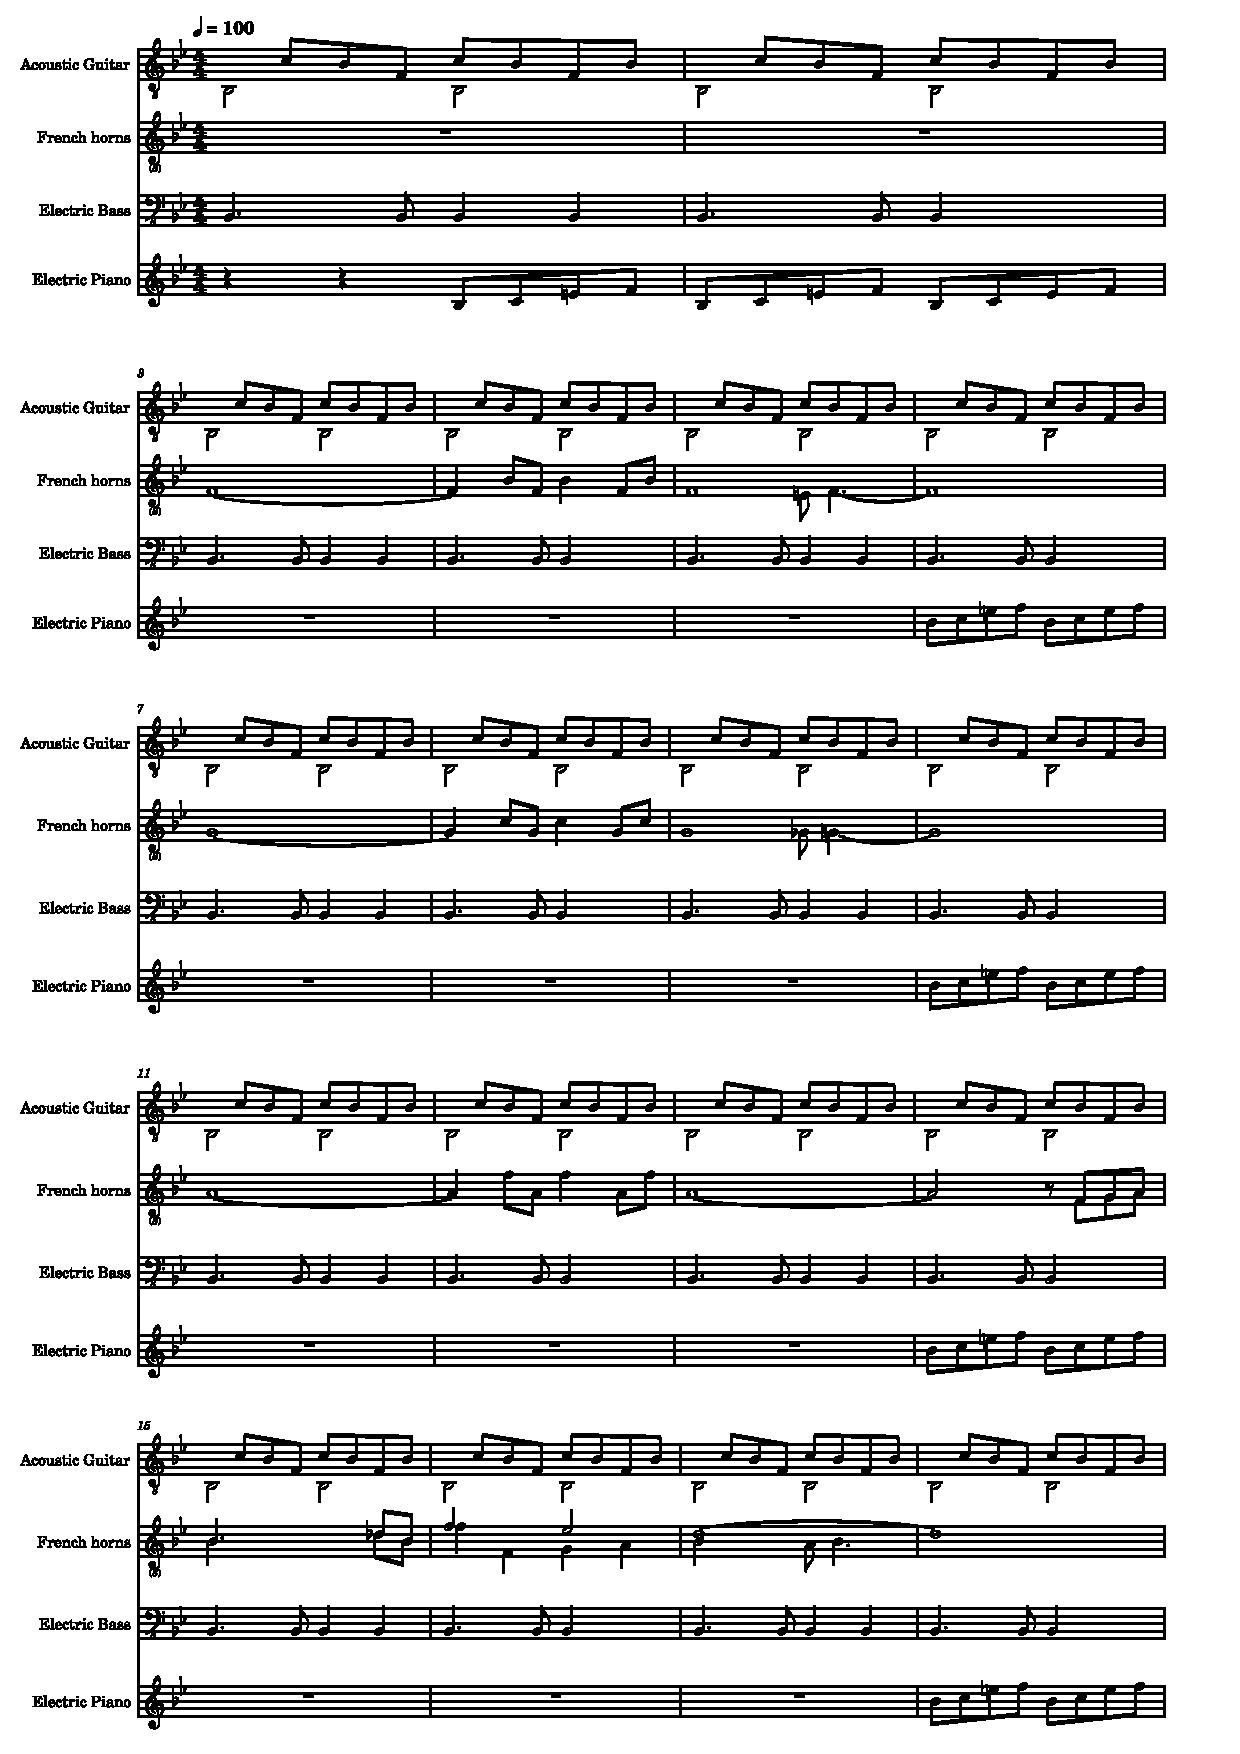
\includegraphics[width=1\linewidth]{img/president-creep-4.pdf}
    \caption{The conclusion of the CREEP Suite sees the combination of all previously heard motifs from the suite's earlier sequences.}
    \label{fig:president-creep-4}
\end{figure}

The acoustic guitar is far more sparse, slow and methodical than the arpeggios heard in ``CREEP Sequence I," which was comparatively more energetic and active.
This mirrors the more systematic and precise work of the reporters as we hear their acousmatic voiceover slowly reading through the names of the list of CREEP employees.
The suspended second adds a subtle layer of tension to the guitar’s otherwise soothing and soporific timbre.
This is complemented by the return of the Lydian motif, performed on an electric piano which provides additional dream-like ethereality.
It thus mirrors the weariness and exhaustion in Woodward and Bernstein's voices as they slowly read aloud the list of names, sounding as if they are about to fall asleep.

This final cue of the CREEP Suite becomes the most expansive of the suite and of the film as a whole with the subsequent addition of two French horns.
Unlike previous cues, however, the horns perform two overlapping motifs: the Alternating Fourths and the Ascending Minor Seconds, performed in a call and response pattern.
This final part of CREEP Suite thus amalgamates aspects from each of the previously heard cues: the Lydian motif; the Minor Second motif; Alternating Fourths; the Polyphonic Melodic run; the Heartbeat bass; and the acoustic arpeggios (Figure \ref{fig:president-creep-4}).
These overlapping, unconnected motifs again point to the complexity of Woodward and Bernstein’s investigation and mirrors their confusion as they exasperatedly discuss the case and argue about the best way to progress.

It simultaneously subtly suggests that the case is beginning to fit together; while the motifs were previously not placed together, here they have been combined in a way that, to the reporters, finally seems to make sense. 
The progress suggested by this successful combination is further alluded to by the electric piano's Lydian motif.
Instead of repeating its four-note motif with no climax, bar 6 of Figure \ref{fig:president-creep-4} sees the motif transposed up an octave to B\flat$_4$, finally seeming to break its endless cycle and progress from its previous pitch.

This is the largest ensemble heard in the entire score, with five instruments and five overlapping motifs.
It is therefore the centrepiece of the score, and accompanies one of the most cinematic shots of the film as a crane shot pulls away from the shot of the reporters in Woodward's car in a crane shot above the city.
The reporters' acousmatic voices continue as the camera seems to float over Washington D.C., much like in the shot accompanying ``Library of Congress,” reinforcing their isolation against, seemingly, the entire power of the Nixon presidency.

The organic instrumentation of the acoustic guitar, electric bass and French horns is contrasted with the other-worldly atmosphere of the electric piano.
Such a combination is not novel to film scoring and can be heard in countless other films.
Yet the combining of such contrasting timbres contributes to a sense of confusion.
The combination of electronic and organic instrumentation was discussed by Donnelly in his examination of \textit{The Fog}.
``The mix of timbres," he writes, ``has the ethereal synthesizer representing the unknown counterposed with the organic sound of the piano that marks the familiar.”\autocites[][156]{donnelly_hearing_2010}
As I have conceded above, these two films function within different genres and \textit{The Fog} was released four years after \textit{President's Men}.
And yet, both films use their scores to create tense and discomforting atmospheres.
Donnelly's analysis can then be transposed onto \textit{President's Men}, as it too presents the spectator with ``familiar" organic instruments in contrast to the ``unknown," ghostly timbre of the electric piano.
Just as it supposedly does in \textit{The Fog}, in \textit{President’s Men }this unfamiliarity comes to also mean the unknown: the truth that the reporters are searching for to make sense of their investigation.


\subsubsection{To Segretti}

While the conclusion of the CREEP Suite suggested progress is finally being made, the next cue presents a much less certain grounding (01:35:25).
This is clearly heard in the lead melody played by the contrabassoon, which performs the slower version of the Perfect Fourth motif, labelled F2 in Figure \ref{fig:president-all-motifs}.
The slower, steadier version of this motif suggests a shift to a more methodical and efficient effort on the part of the reporters, much as the acoustic guitar arpeggio from ``CREEP Sequence IV."
It mirrors the dialogue between the reporters as they examine the evidence they have uncovered related to a new witness, Donald Segretti, and his connection to Watergate.
This forces them to rethink the case and the assumptions they had previously made:
\begin{quote}
Bernstein: If the break in was just one incident in a campaign to sabotage that began a whole year before Watergate-

Woodward: Then for the first time the break in makes sense.

Bernstein: This isn’t so crazy. This whole thing didn’t begin with the bugging of the headquarters.

\end{quote}
The cue ends abruptly as Bernstein knocks on Segretti’s door to interview him.


\subsubsection{Paranoia Walk}

The ominous, paranoid atmosphere that is pervasive through \textit{President’s Men}, and mirrors the general sense of distrust that was rife during the decade, is most explicit in the score as Woodward makes his way home from another meeting with Deep Throat (01:42:55).
This cue enters after their meeting is cut short when they are startled by nearby a car starting its engine.
The camera cuts to see the car driving away before cutting back to Woodward, watching the car over his shoulder before turning back to Deep Throat, only to realise that he has vanished.
A cut to a wide shot reveals that Woodward is standing alone in the car park.
The cue begins when Woodward begins to leave.

Unlike previous cues, this cue features very little melodic movement, instead consistently entirely of low, sustained drones played by piano, acoustic guitar, electric bass guitar, electric piano and a cello.
Each instrument simply plays a low C, sustained over multiple bars.
These pedals heighten the tense atmosphere and echoes Woodward's paranoia as he makes his way home, convinced that he is being followed.
The electric piano then introduces the Sustained Ascending Electric Piano motifs, H1 and H2 in Figure \ref{fig:president-all-motifs}.

As with the previous use of the electric piano, the sequence is imbued with a mystical, dream-like timbre from the electric piano's tremolo, adding a surreal quality to the scene.
As if in response to the music and its sinister atmosphere, Woodward hurries his pace, fearing that he is being followed.
Once the piano completes its eight-note sequence, we are left with just the droning bass instruments and an intermittent Heartbeat bass line.
This minimal instrumentation, along with Woodward’s footsteps on the pavement, highlighting his isolation in this potentially dangerous situation.
The music swells to a crescendo, increasing the scene's intensity until it stops abruptly as Woodward spins around, expecting to see his pursuer, only to realise that there is nobody there.
It is perhaps in this cue that the psychological effects of the music are most keenly felt, as the music's consistent drones and ultimate crescendo reflects Woodward's increased paranoia and belief that he is being stalked.
In this, it subsequently heightens the anxiety felt by the spectator.
The dreamy quality of the electric piano is thereby retroactively imbued with an additional meaning: it begins to represent Woodward’s imagination running away with him as he realises that, in this instance at least, his paranoia was unnecessary.

Shire's used of repetition, low drones, and unfamiliar timbres is most at play in this brief cue, and each of these aspects combine to create a disturbing sense of discomfort. 
In evoking this sense, Shire draws upon the audience’s assumed cineliteracy to make them except a jump scare following the cue’s crescendo.
However, when he turns around, it becomes apparent that both Woodward and the audiences’ paranoia was misplaced.
This acts to heighten the audience's sense of confusion and lack of security as the villain that haunts both the film and the nation's psyche is absent while seemingly omnipresent.




\subsubsection{To Deep Throat II}

Woodward again returns to Deep Throat soon after this sequence.
The next cue is introduced as he rushes to the usual car park, having fallen asleep and almost missed the appointment (02:00:38).
This cue begins just as ``Paranoia Walk” does, with repeated, sustained bass tones.
Woodward leaves his apartment and finds a taxi but, before he can get in, he notices a car pulling up in front of him (Figure \ref{fig:president-frenzied-intro}).
The electric piano returns as Woodward watches this second car park near him, introducing the Frenzied Piano motif.

The rapid tempo and  high pitch of this motif reflects Woodward's manic rush to get to his meeting with Deep Throat in time.
Further, as I noted above, this Frenzied motif mirrors scoring practices heard in horror films both before and after \textit{President's Men}'s release.
The cue therefore draws upon established generic tropes to create a sense of dread, anxiety, and fear, appropriate for the paranoia that Woodward and the spectator felt during this period.
The horror in this instance is not just the threat to Woodward's safety, but the threat to his personal freedoms which the unseen governmental forces are apparently seeking to curtail.
In pursuing the story, Woodward is thus risking elements fundamental to his American identity, and the music reinforces the tragedy of this situation.

Woodward gets into the taxi and they drive away as the French horn's Ascending Minor Second motif returns.
As the taxi drives away from the camera, the shot lingers on the parked car which does not move, highlighting Woodward's misplaced paranoia; while he perceives threats at almost every turn, he never directly faces one.
The Minor Second motif is succeeded by the Hunting Fanfare which again alludes to the simultaneous notion of the reporters hunting the story while being hunted themselves.

At this point in the film Woodward and Bernstein are coming close to finally uncovering the full story, and, as a result, the sense of paranoia is at its highest.
This increases the tension and the stakes of ``the hunt."
When combined with the Frenzied Piano's association with horror scoring and the threat to the reporters that this represents, the suggestion here is that the reporters are the hunted, rather than the hunters.

As the targets of the government's hunt, Woodward and Bernstein's patriarchal, individualistic American identity is under threat.
Throughout the film, these attributes have allowed the reporters to successfully pursue the Watergate story.
They have also, however, led them to uniquely dangerous situations, as the government is supposedly attempting to suppress these rights.
The score tells us that self-sufficient, individualist, patriarchal freedom is such a fundamental aspect to the American identity that any threat to it is tantamount to the sort routinely seen in the horror genre.
\begin{figure}
    \centering
    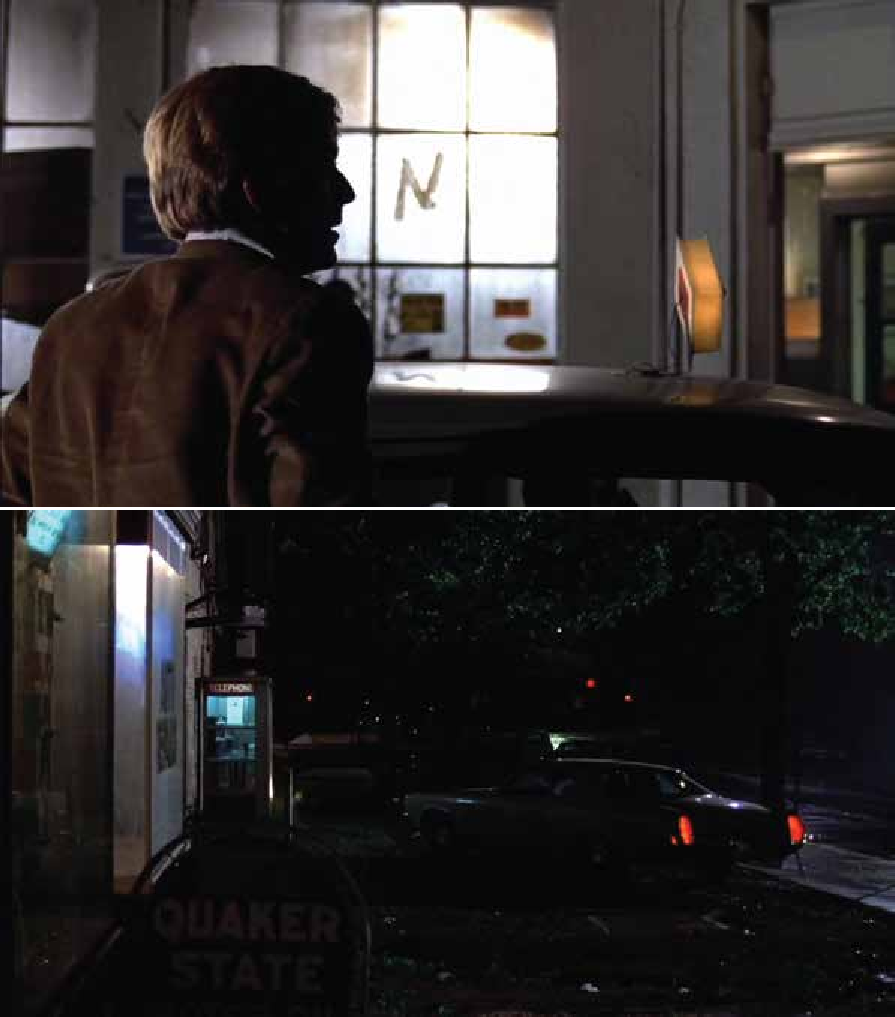
\includegraphics[width=0.5\linewidth]{img/president-frenzied-intro.pdf}
    \caption{While travelling to his meeting with Deep Throat, Woodward looks up and sees a car pull up in front of him. As the car parks, the Frenzied Piano motif is introduced.}
    \label{fig:president-frenzied-intro}
\end{figure}

The cue is brought to a gradual end with the electric piano slowly its arpeggio patterns before concluding with the Sustained Ascending motif.
Over this four-note pattern – rising through a major third, a minor sixth, and a perfect fourth – the motif ascends a perfect eleventh, opening on the cue's root of E\flat, and ending on A\flat.
This cue deviates from the previous use of this motif, heard in ``To Deep Throat," as it does not feature the corresponding, alternative motif, labelled H2 in Figure \ref{fig:president-all-motifs}.

Rather than an entirely ascending pattern, the alternative iteration of this motif includes a descending minor sixth between the second and third notes.
By foregoing this descending interval, the motif here evokes a more optimistic ambience through its use of large intervallic ascents.
The slightly more uplifting tonality of the ascending motif contrasts the ominous nature of the Frenzied Piano and the Hunting Fanfare by alluding to how close the reporters are to completing their goal and uncovering the truth.

During Woodward and Deep Throat's meeting, there is evident tension between the two men as the reporters had recently written a story associating Nixon's Chief of Staff H.R. Haldeman with the Watergate scandal 
without sufficient evidence to back up their claims.


This error, Deep Throat claims, ``put the investigation back months."
Frustrated with Deep Throat's cryptic clues about the truth of the scandal, Woodward insists that he share the full story.
After a long pause, Deep Throat concedes and discloses what he knows and, for the first time, Woodward realises the scale of the scandal:
\begin{quote}
It involves the entire US intelligence community. FBI, CIA, Justice. It's incredible. The cover up had little to do with watergate, it was mainly to protect the covert operations. It leads everywhere. ... Your lives are in danger.
\end{quote}
The scene ends with this revelation and the next scene begins with Woodward arriving at Bernstein's apartment where he shares what he just learnt.
They both then go to \textit{Washington Post} editor, Ben Bradlee's, house to tell him directly what they have both discovered.

\subsubsection{Bradlee Lawn}

The final cue is heard at the end of this scene, where the reporters speak to Bradlee in front of his house in the middle of the night.
The reporters here lay out all they have learnt about the full scale of the scandal, while Bradlee counters by explaining the pressure they are under since the mistake they made in misidentifying some co-conspirators.
He then sarcastically details the stakes of the investigation:
``Nothing's riding on this except the first amendment to the Constitution, freedom of the press, and maybe the future of the country."\autocites[The first amendment of the USA's Constitution declares that ``Congress shall make no law respecting an establishment of religion, or prohibiting the free exercise thereof; or abridging the freedom of speech, or of the press; or the right of the people peaceably to assemble, and to petition the Government for a redress of grievances."][]{noauthor_constitution_nodate}

The camera cuts to a wide shot of the three men following Bradlee's monologue, as if they are being watched from across the street.
After several seconds, the reporters walk away and a bass pedal opens the cue before it is joined by a bass clarinet performing a slow-tempo version of the Perfect Fourth motif.
Following Bradlee's mention of the USA's constitution, the patriotic allusion of this motif, through its Coplandesque repetition of the perfect fourth intervals, is far more overt.
The motif therefore restates the reporters' embodiment of Turner's American identity.

The motif's mode-preserved transpositions are mirrored in the cello's pedal bass, providing a perfectly consonant accompaniment.
The contrabassoon deviates from its motif, however, with a four-note passage (bars 5-6 in Figure \ref{fig:president-bradlee-lawn}).
Again, this motif remains fully diatonic.

\begin{figure}
    \centering
    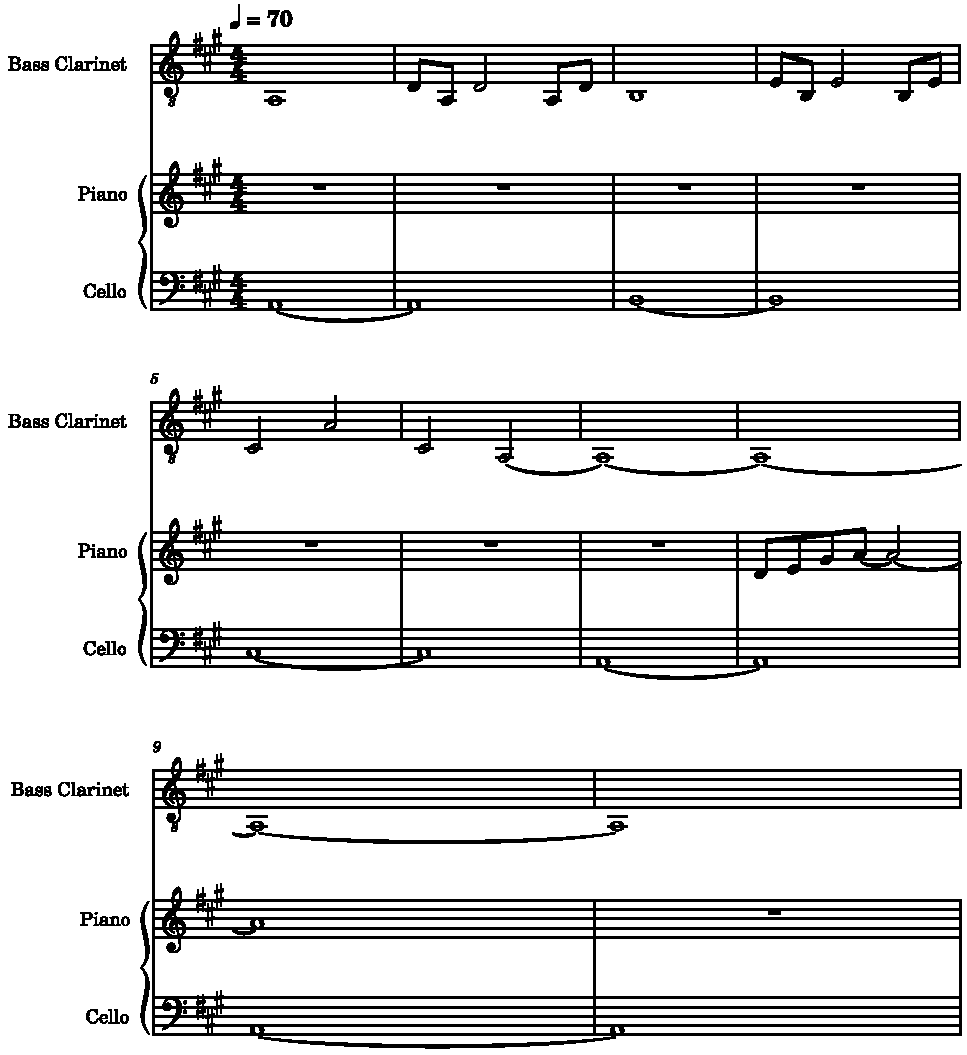
\includegraphics[width=0.5\linewidth]{img/president-bradlee-lawn.pdf}
    \caption{The final cue heard in \textit{President's Men}.}
    \label{fig:president-bradlee-lawn}
\end{figure}

As the contrabassoon concludes its motif on a sustained C\sharp, the piano plays the Lydian motif for a single ascending run, ending on the root A.
Although this is the sixth cue that this motif is heard in, this instance provides a substantial, if subtle, difference:
while the motif's augmented fourth adds a layer of non-diatonicism to the other cues that it is heard in, the augmented fourth in this case is a G\sharp, the major seventh of the A major scale.
As such, this motif, while still functioning within the D Lydian mode, is entirely diatonic within the key of A major.
This removes the sense of dissonance that it had created in its previous cues, and therefore reduces the sense of discomfort that it generated.
Furthermore, as it is performed just once before sustaining its final note, the motif seems to finally has reached its climax which, in this case, is the cue's tonal centre.
This provides the spectator with a delayed sense of resolution to the previously tonally ambiguous and ominous motif, mirroring the reporters' sense of accomplishment.
\begin{figure}
    \centering
    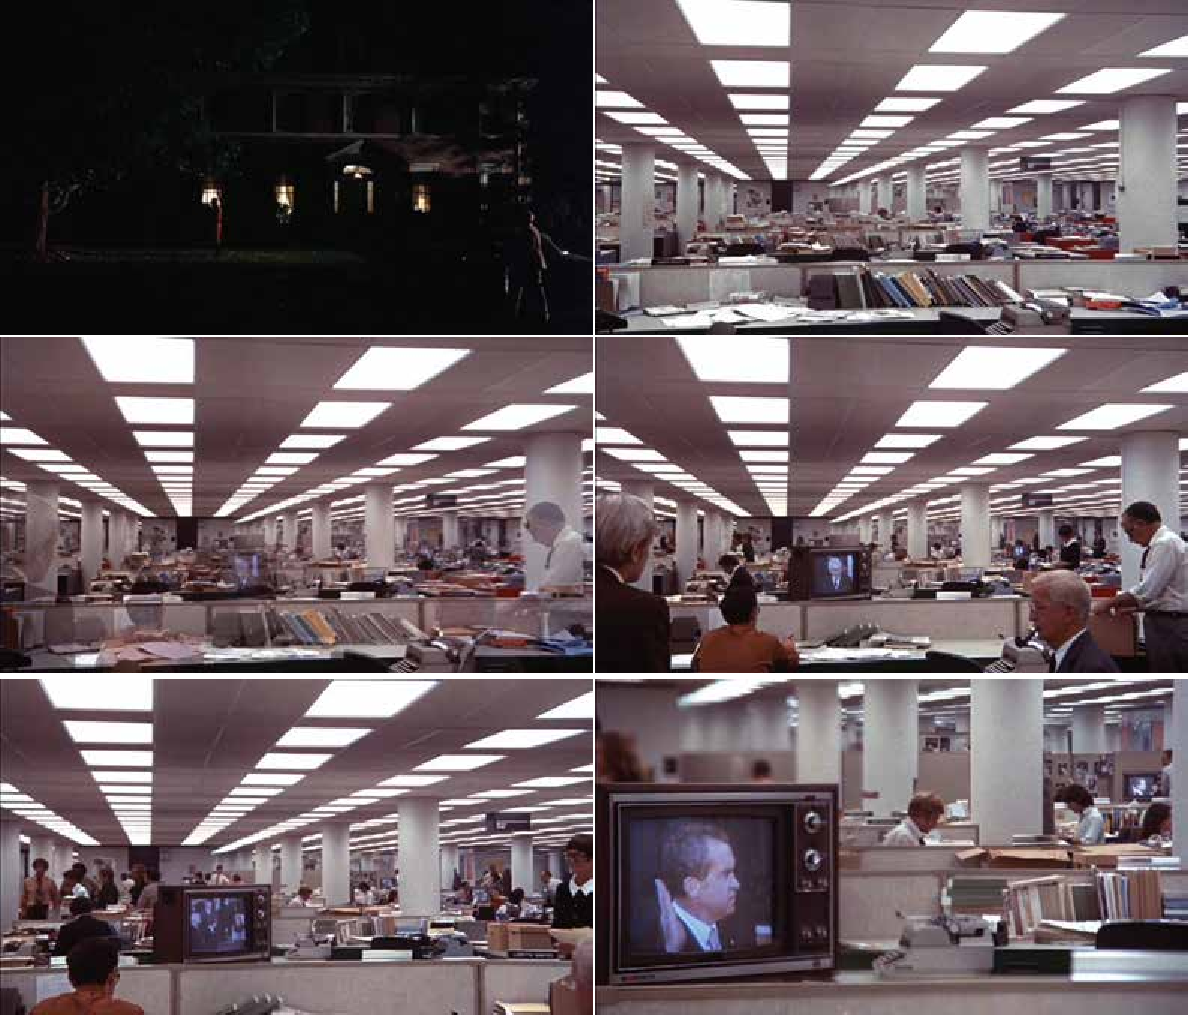
\includegraphics[width=0.5\linewidth]{img/president-ending-dissolve.pdf}
    \caption{An abrupt cut from an external shot of Woodward and Bernstein leaving Ben Bradlee's house to the interior of the \textit{Washington Post} newsroom. The reporters can be seen in the middle distance as a dissolve introduces more of their colleagues gathered round a television showing Richard Nixon's 1975 inauguration.}
    \label{fig:president-ending-dissolve}
\end{figure}

The scene ends with an abrupt cut to the interior of the newsroom.
The darkness of the reporters' late-night meeting with Bradlee – wherein they discuss the government's sinister machinations – is sharply contrasted with the office's harsh fluorescent lighting.\autocites[The use of fluorescent lights was another decision made to replicate the exact look and feel of \textit{The Washington Post}'s newsroom. As cinematographer Gordon Willis writes: ``Prior to construction, the lighting was discussed at length and, since the real newsroom is lit exclusively with fluorescent lamps, my feeling was to keep it just that way. Fluorescent has a look all its own and I wanted to retain that look. So, fluorescent it was."][]{willis_photographing_2019}
Woodward and Bernstein are barely visible at their desks in the middle distance, while the sound of their typewriters are foregrounded in the sound mix, competing for prominence with the contrabassoon's Perfect Fourths.

After the Lydian motif is performed, the cue slowly fades out in sync with a dissolve to a much busier office.
A television is placed on a desk and a group can be seen watched another screen, out of shot, showing Richard Nixon's 1975 inauguration.
The camera slowly begins to zoom in, not on the television screen, at it initially seems, but on Woodward and Bernstein who remain in the centre of the shot throughout the sequence (Figure \ref{fig:president-ending-dissolve}).
I will discuss the significance of the constant sound of the typewriters below, but it is important to note here how they fully replace the score, signifying the reporters' focus on uncovering the scandal as they continue their reportage almost oblivious to the historic occasion unfolding on the television screens surrounding them. 

The Coplandesque Perfect Fourth motif, accompanying the image of the reporters, unconcerned with the inauguration's pageantry, calls to mind Copland's ``Fanfare for the Common Man," which I discussed above in relation to Shire's Hunting Fanfare.
An allusion to Copland's piece seems appropriate, given its original intention as a means to celebrate patriotic fervour and the image and sound of Richard Nixon's inauguration that enters as soon as the cue fades out.
The use of the motif here, taken with its representation of the American identity, could be read as an uncritical and apposite accompaniment to the patriotic signing in of a new president.
However, this allusion to the American identity becomes loaded with irony considering everything that Woodward and Bernstein have uncovered, and as they continue their work that will ultimately lead to President Nixon's resignation.
Instead of a complementary accompaniment to the celebration of the president, the celebratory American identity is not attributed to the presidential administration but to the two reporters who have worked diligently and proven their worth as individualistic, patriarchal American heroes.

 

\subsubsection{Cue Conclusions}

As we have seen through this analysis of each of \textit{President's Men}'s cues, tonal ambiguity is a fundamental aspects of the score.
Although, each of the cues recycle the same few motifs laid out in Figure \ref{fig:president-all-motifs}, there is rarely a definitive suggestion of a diatonic centre. 
Shire instead makes consistent use of modes to create a lack of stable diatonicism which in turn denies the spectator a familiar and comforting sense of consonance.
This reflects the paranoia and lack of security that was endemic in the United States at this time, as detailed in Christensen's discussion of the nation's post-traumatic period.

By arranging the various motifs in different combinations throughout each cue, the score reflects the story the reporters are investigating as they attempt to make sense of a scandal that refuses to fit into a coherent  narrative.
As the reporters work to make sense of the case, they are often left to make sense of information that does not offer any simple conclusions, similar to how the score does not cohesively adhere to any clear diatonic tonality

Having discussed \textit{President's Men}'s non-diegetic soundtrack, I will now turn to the film's diegetic soundworld.
As I will detail below, this provides an equally significant representation of the film's themes.



\subsection{Diegetic Soundworld} - i think will move this up to between section on themes and motifs.

As I referenced above, the recreation of a believable, working office was very important to the filmmakers.\footnote{Robert Redford, who in addition to portraying Bob Woodward also bought the rights to the book and used his production company to help make the film, initially intended on making the film a documentary. While Alan Pakula dissuaded him from this idea, the grounded, documentary aesthetic is still keenly felt throughout the majority of the film.}
This attempt at realism is overt in the film's diegetic soundworld.




The film opens on what appears to be a plain grey screen and lingers on this static shot for roughly 16 seconds.
A series of letters are then stamped onto what we now understand is a piece of paper in a typewriter.
The date `` June 1, 1972" is written onto the page, establishing the film's temporal setting as well as foreshadowing the importance of the typewriter and reportage (Figure \ref{fig:president-opening-type}).

\begin{figure}
    \centering
    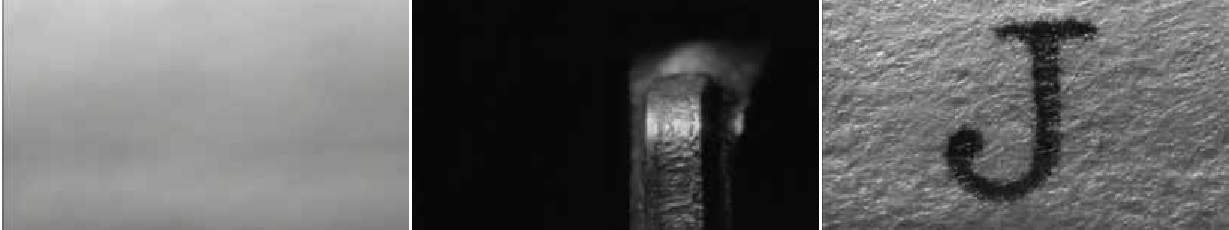
\includegraphics[width=0.5\linewidth]{img/president-opening-type.pdf}
    \caption{The opening shot of \textit{President's Men} sees an extreme close-up on a blank piece of paper before a typewriter begins to type the day's date, establishing the setting and the importance of reportage.}
    \label{fig:president-opening-type}
\end{figure}

Once the date is written, a new line is set and the shot cuts to archival footage of President Nixon's helicopter landing in Washington D. C., prior to his State of the Union address.
As Nixon's helicopter lands, he enters the the Chamber of the House of Representatives, while the television newsreader Walter Cronkite narrates his movements.
The camera lingers on President Nixon's smiling face as he looks over the room and almost the entire U.S. government.
The film's opening two minutes therefore establish the importance of the news and media industries, in addition to the quasi-documentary aesthetic.

The shot of Nixon's face slowly fades to black and the applause is replaced by Spanish voices and a scratching sound as the film's title sequence begins.
The scratching sound is revealed as the lock to the Democratic National Committee headquarters being picked.
The next sequence depicts the burglars breaking into the DNC office and occurs in almost complete silence other than their voices and the distant sound of traffic.
Nearby police officers are alerted to the break-in and find and arrest the burglars.
The scene ends with an abrupt edit, from the burglars with their hands raised in almost total darkness, to the brightly-lit newsroom.
This contrast between the darkness in which the burglars are operating and the bright newspaper office presents an overt reference to the reporters' attempts to bring the shadowy criminal activity into the light, while the complete lack of any score and minimal dialogue reinforces the film's attempts at verisimilitude. 

\textit{Washington Post} managing editor Howard Simons (Martin Balsam) is seen walking across the newsroom to the office of Harry Rosenfeld (Jack Warden), another of the paper's editors, where they discuss the details of the break-in.
This scene, and every scene that takes place in the newspaper's office – with the exception of the final cue, ``Bradlee Lawn," as I will discuss below – does not feature any non-diegetic score.
It is instead filled with the sound of typewriters which provide a near-constant soundscape, and are perhaps the most important sound heard throughout the film.
These machines are the first sound that is heard, in the opening sequence depicted in Figure \ref{fig:president-opening-type}.

One example in which this soundscape is particularly significant is an early scene in Rosenfeld's office .
Woodward tells the team what he discovered at the burglars’ arraignment hearing (00:11:48).
The typewriters are clearly heard despite being in a completely different room.
The typewriters prove highly audible, as their harsh, percussive timbres envelope the spectator into the film’s diegesis and are key in creating the sense that this is a real, functioning newspaper office.
This follows Kevin Donnelly’s suggestion that ``sounds in film exist essentially to bolster or `make real’ the images we see on screen and the surrounding world we imagine.”\autocites[][108]{buckland_saw_2009}

In scenes where the audience’s belief in the diegesis is paramount, the narrative is left to unfold without any non-diegetic accompaniment.
The soundtrack is instead filled with ambient noise emitting from within the film’s diegesis: cars and planes passing making the reporters need to raise their voice to speak to each other; the background chatter of passers-by; the sound of a neighbour cutting their grass.
This is often referred to as location or direct sound, described by Michel Chion as ``sounds recorded during filmmaking [which are] enriched by later addition of sound effects, room tone, and other sounds.”\autocites[][96]{chion_audio-vision_1994}
The use of location sound to create a more ``realistic” diegesis was a common trend throughout the New Hollywood period and is evident in films such as \citetitle{altman_msh_1970} (Robert Altman, 1970), \citetitle{altman_long_1973} (Robert Altman, 1973) and \citetitle{lumet_dog_1975} (Sidney Lumet, 1975), where characters are often forced to raise their voices substantially to be heard, or even have their voices drowned out entirely by background noise.

While these three films each evince location sound in an edited and highly controlled manner, there were also more experimental and less mainstream films that made prominent use of location sound.
Charles Burnett’s \citetitle{burnett_killer_1978} (1978) is one such example.
For Paula J. Massood, \textit{Killer of Sheep}’s location sound demonstrates Burnett’s “Third Cinema, documentary, and neorealist influences,” and contributes to “creat[ing] a unique form of cinematic realism."\autocites[][39]{massood_aesthetic_1999}

For Massood, ``the use of direct sound combined with location shooting provides the films produced by the L.A. School [the group of UCLA graduates from which Burnett emerged] with a sense of documentary realism. … Burnett takes first-hand observations of his environment and transposes them into a fictional narrative that is documentary in both look and sound."\autocites[][27]{massood_aesthetic_1999}
Massood’s discussion here, although specifically focussed on the socio-political context that Burnett was responding to, can be extended to \textit{President’s Men} which uses similar techniques to depict a narrative that aesthetically resembles a documentary through its use of location sound, location shooting, and free-flowing, naturalistic dialogue.
These techniques combine to create a realist – if not necessarily ``realistic" – diegesis that is key in reinforcing that the film is depicting a true story and, subsequently, pointing to the culpabilities of individuals in the Nixon administration and potential fallibilities of those in power more generally. 

The realist nature of \textit{President’s Men}’s sound extends to the newsroom’s fluorescent lighting which bathe the offices in an unglamorous light, replicating the real lighting of \textit{The Washington Post}'s newsroom.
In addition to adding a sense of verisimilitude, this \textit{mise-en-scène }also contributes a strong thematic subtext. Mark Feeney writes in \textit{Nixon at the Movies} that this ``remorseless illumination … [conveys] reassurance and fidelity to the truth,” and asks “what better antidote for paranoia than glare? It deprives enemies of any shadows to lurk in.”\autocites[][263]{feeney_nixon_2004} 
A similar message is portrayed in the ever-present sound of typing.
The cacophonous wall of noise generated by the typewriters insinuates the same devotion to rooting out the truth and mimics the seemingly tireless efforts and determination of the journalists that, the film tells us, will ultimately uncover the criminal wrongdoing within the government and hold those in power accountable.
In this, the typing underlines the film’s themes of journalistic integrity and freedom of the press, which extends to the reporters' individual entrepreneurialism.
However, the typing also provides a sense of uneasiness: with their non-stop tapping, the typewriters at times overwhelm the diegesis and compete with the reporters’ conversations for prominence in the soundtrack.
This arrhythmic, high-pitched tapping is highly audible and therefore impossible to ignore, escalating the tension with its grating timbre and unavoidable placement in the soundtrack. 


The audibility of typewriters is most notable in the scene leading to Woodward and Bernstein’s first proper introduction (00:19:14).
This scene plays out for several minutes without any dialogue, only the distant chattering of unseen colleagues.
These colleagues further add to the soundscape through their uninterrupted typing throughout the screen.
This noise is the principal source of sound until Woodward approaches Bernstein.
In this, the typing is used in a similar way to a non-diegetic score, providing what Ben Winters may call ``wallpaper … [lending] itself to characterising the nature and feeling of the space in which the action takes place” as it contributes to the notion that this is a real, functioning office.\autocites[][43]{winters_musical_2012}
Winters discusses the idea that film music does not actively “narrate” a story, but rather ``unscroll[s] \textit{as part of }the narrative, tracing its contours mimetically.”\autocites[][41]{winters_musical_2012}
While Winters’ focus is on non-diegetic music, it provides a useful analogue here;
\textit{President’s Men}’s typewriters do not directly narrate the film’s story yet provide an atmospheric underpinning and reinforces its themes, as mentioned above.

The typewriters’ ``fidelity to the truth,” to borrow Feeney’s expression, is underlined here in their endless typing as they maintain their steady pace regardless of the narrative action on screen, thereby evoking their indifference to the interpersonal squabbles of the two main characters and highlighting their sole interest in pursuing the news.
In this, we are reminded of the theme that, regardless of distractions or barriers, the press will persist, while the president’s men, too, remain persistent in their attempts to side-track the reporters’ investigation/

\textcolor{red}{V GOOD! A BIT REPETITIVE/COULD BE COMPRESSED/WEE BIT REORGANISED ULTIMATELY, BUT V GOOD
While this use of diegetic sound contributes both verisimilitude and thematic consonance, another element of the soundtrack that is worthy of analysis is the acousmatic voice.

Also need to figure out where to add other diegetic elements, think about the music heard during Nixon's inauguration; the classical music they use to drown out the bug in the scene right between Bradlee Lawn.}




\subsection{The Voice}

Acousmatic voices are those that we hear without seeing their source.
Such voices play a key role in \textit{President’s Men} as Woodward and Bernstein conduct their investigation into the various figures purportedly linked to the Watergate break-in, an investigation that largely takes place through phone calls to unseen figures.
Michel Chion states that the invisibility of the acousmatic voice grants it ``magical powers”: ``ubiquity, panopticism, omniscience and omnipotence.”\href{applewebdata://3A1D666A-D52A-46D2-8C90-343A1EE58F85\#_ftn1}{\textsuperscript{\textsuperscript{[1]}}} \href{applewebdata://3A1D666A-D52A-46D2-8C90-343A1EE58F85\#_msocom_3}{[AD3]}
While the acousmatic voices heard in \textit{President’s Men} are undoubtedly grounded within a non-supernatural world, as foregrounded in the film’s documentary style, their sources emit different sorts of power:
literally, in the sense that they are often the voices of high-ranking government officials;
and metaphorically, because their power is the secret information regarding the administration’s wrongdoings.
As they continue to investigate the story, the reporters attempt to uncover these secrets from disembodied voices; thereby attempting to wrestle the power associated with the acousmatic voices away from their sources as they, wittingly or unwittingly, divulge key information that Woodward and Bernstein will use to build their story\href{applewebdata://3A1D666A-D52A-46D2-8C90-343A1EE58F85\#_msocom_4}{[AD4]} \href{applewebdata://3A1D666A-D52A-46D2-8C90-343A1EE58F85\#_msocom_5}{[CW5]} \href{applewebdata://3A1D666A-D52A-46D2-8C90-343A1EE58F85\#_msocom_6}{[AD6]} .
Many of these voices are de-acousmatised as the reporters begin to conduct interviews in person, yet, when granted corporeality these voices lose the ostensible powers Chion cites but none of the actual power that Woodward and Bernstein are attempting to gain\href{applewebdata://3A1D666A-D52A-46D2-8C90-343A1EE58F85\#_msocom_7}{[AD7]} \href{applewebdata://3A1D666A-D52A-46D2-8C90-343A1EE58F85\#_msocom_8}{[CW8]} \href{applewebdata://3A1D666A-D52A-46D2-8C90-343A1EE58F85\#_msocom_9}{[CW9]} . \href{applewebdata://3A1D666A-D52A-46D2-8C90-343A1EE58F85\#_msocom_10}{[AD10]} 

While Woodward and Bernstein use their own voices to extract information and power from various witnesses to accrue a power that will ultimately bring down many figures within the Nixon White House, towards the end of the film we see that their attempted weaponisation of the \href{applewebdata://3A1D666A-D52A-46D2-8C90-343A1EE58F85\#_msocom_11}{[AD11]} \href{applewebdata://3A1D666A-D52A-46D2-8C90-343A1EE58F85\#_msocom_12}{[CW12]} \href{applewebdata://3A1D666A-D52A-46D2-8C90-343A1EE58F85\#_msocom_13}{[CW13]} voice is turned against them.
As Woodward meets his source, Deep Throat, we learn that the reporters are being watched and that their lives are in danger (02:01:05).
Following this scene, Woodward rushes to Bernstein’s home to warn him that they have likely been bugged, and the two of them then go to editor Ben Bradlee’s home to deliver the same message.
In this, we see a reversal of power dynamics; while the reporters had previously worked to expose the truth through coaxing information from often acousmatic voices, now they find themselves in a position where their own acousmatic voices are being used against them and have potentially put their lives at risk.
As such, the weapon that the reporters had primarily been relying on thus far, the voice, is now being turned on themselves, subsequently implying that their own voices have turned them into the hunted rather than the hunters\href{applewebdata://3A1D666A-D52A-46D2-8C90-343A1EE58F85\#_msocom_14}{[AD14]} \href{applewebdata://3A1D666A-D52A-46D2-8C90-343A1EE58F85\#_msocom_15}{[CW15]} . GOOD – clearer

Deep Throat’s voice is also worthy of consideration when discussing acousmatic voices\href{applewebdata://3A1D666A-D52A-46D2-8C90-343A1EE58F85\#_msocom_16}{[AD16]} \href{applewebdata://3A1D666A-D52A-46D2-8C90-343A1EE58F85\#_msocom_17}{[CW17]} .
The dark, shadowy car park where his late-night meetings with Woodward take place presents a sharp contrast to the brightness of the newspaper offices (00:35:35; 01:39:29; 02:01:50).
This darkness falls dramatically across Deep Throat’s face, masking him in shadow and helping to hide his identity. While we can make out the outline of his face, his voice almost becomes acousmatic.
Although it is not fully acousmatic, and therefore not necessarily imbued with the powers that Chion discusses, the dialogue nevertheless implies that Deep Throat is literally omniscient as he appears to know every detail of the story that Woodward and Bernstein are reporting.

Deep Throat’s voice is granted additional weight in the way is it presented during his meetings with Woodward.
These scenes play out without any non-diegetic scoring while the diegetic soundscape is treated in a realistic manner, much like the scenes set within the newspaper offices:
Woodward’s footsteps echo throughout the car park;
offscreen, we hear the screeching tires of distant cars;
a constant room tone that we could perhaps assume is emitting from an unseen generator but, regardless of its source, contributes what Isabella van Elferen may describe as “an uncomfortable buzz of white noise.”\href{applewebdata://3A1D666A-D52A-46D2-8C90-343A1EE58F85\#_ftn2}{\textsuperscript{\textsuperscript{[2]}}}
Such aural occurrences contribute to creating a believable film world, while the room tone helps to maintain the sense of unease felt through the narrative.

This tension is furthered as Woodward and Deep Throat discuss the case in hushed tones that we can clearly hear.
This conversation presents, as Frances Dyson writes, “impossibly intimate sounds … [voices] too large for any body” and draws us almost uncomfortably close to the characters.\href{applewebdata://3A1D666A-D52A-46D2-8C90-343A1EE58F85\#_ftn3}{\textsuperscript{\textsuperscript{[3]}}}
Lisa Coulthard has also discussed this somewhat generic cinematic technique, writing that “voices, breath, or small inconsequential sounds have a volume, presence, and impact far beyond what would exist in everyday life.”\href{applewebdata://3A1D666A-D52A-46D2-8C90-343A1EE58F85\#_ftn4}{\textsuperscript{\textsuperscript{[4]}}}
However, what is more uncommon here is the foregrounding of what Coulthard calls “mouth sounds,” most prominently heard as Deep Throat’s saliva as he chews and swallows between sentences.\href{applewebdata://3A1D666A-D52A-46D2-8C90-343A1EE58F85\#_ftn5}{\textsuperscript{\textsuperscript{[5]}}}
Coulthard discusses this phenomenon with particular regard to both violent and intimate kissing scenes, both of which provoke what she terms “acoustic disgust” through the foregrounding of sounds she describes as “moist,” “gross” and “squishy.”\href{applewebdata://3A1D666A-D52A-46D2-8C90-343A1EE58F85\#_ftn6}{\textsuperscript{\textsuperscript{[6]}}}
In this instance, the disgust is caused through the close miking of both characters which allows us to hear their mouth sounds, specifically Deep Throat’s. Coulthard terms this an “auditory close-up,” a technique that can “[intensify] an uncomfortable intimacy that veers into disgust.”\href{applewebdata://3A1D666A-D52A-46D2-8C90-343A1EE58F85\#_ftn7}{\textsuperscript{\textsuperscript{[7]}}}
Following Coulthard’s terminology, we are placed within an uncomfortable proximity to Deep Throat, where we can clearly hear “the sound of the body itself, its materiality and moisture [which] is where sonic disgust thrives.”\href{applewebdata://3A1D666A-D52A-46D2-8C90-343A1EE58F85\#_ftn8}{\textsuperscript{\textsuperscript{[8]}}}

The discomfort that this “disgust” evokes \href{applewebdata://3A1D666A-D52A-46D2-8C90-343A1EE58F85\#_msocom_18}{[AD18]} \href{applewebdata://3A1D666A-D52A-46D2-8C90-343A1EE58F85\#_msocom_19}{[CW19]} \href{applewebdata://3A1D666A-D52A-46D2-8C90-343A1EE58F85\#_msocom_20}{[CW20]} retains a thematic consonance with the tension prominent throughout the film.
In placing the point of audition so close to Deep Throat’s mouth, we are provided no release from the tension of the dramatic narrative;
rather, as Martine Beugnet writes, “the \href{applewebdata://3A1D666A-D52A-46D2-8C90-343A1EE58F85\#_msocom_21}{[AD21]} \href{applewebdata://3A1D666A-D52A-46D2-8C90-343A1EE58F85\#_msocom_22}{[CW22]} audio close-up pulls the viewer in and envelops him or her with a sensuous or uncanny sense of intimacy or gives full power to the feelings of repulsion brought forth by excessively close contact.”\href{applewebdata://3A1D666A-D52A-46D2-8C90-343A1EE58F85\#_ftn9}{\textsuperscript{\textsuperscript{[9]}}}
In her book, Beugnet focuses on sensuality within French film predominantly from the late 20\textsuperscript{th} and early 21\textsuperscript{st}centuries, noting that “recent French cinema offers particularly vivid illustrations of how such techniques have the potential of radically renewing our experience of watching, sensing and thinking through film.”\href{applewebdata://3A1D666A-D52A-46D2-8C90-343A1EE58F85\#_ftn10}{\textsuperscript{\textsuperscript{[10]}}}
Despite the specificity of her study, it remains applicable in the case of \textit{President’s Men} as the repulsion and “uncanny intimacy” of the auditory close-up maintains the sense of uneasiness felt by the generic “thriller” aspects of the film.
Furthermore, through the atmospheric use of non-diegetic scoring, the soundtrack maintains the film’s theme and sense of the post-traumatic cycle by denying the audience any opportunity for a release of the tension. \href{applewebdata://3A1D666A-D52A-46D2-8C90-343A1EE58F85\#_msocom_23}{[AD23]} 

I have thus far solely discussed the use of diegetic sound in \textit{President’s Men}; however, of equal interest to my study is the use of non-diegetic scoring.
While scoring is only seldom used, I will now provide a cue-by-cue analysis of the score to explore non-diegetic instances of musical representation of the film’s themes and subtext.
In doing so, I refer to the titles of certain cues as they relate to the soundtrack album released in 2007.\href{applewebdata://3A1D666A-D52A-46D2-8C90-343A1EE58F85\#_ftn11}{\textsuperscript{\textsuperscript{[11]}}}

\href{applewebdata://3A1D666A-D52A-46D2-8C90-343A1EE58F85\#_ftnref1}{\textsuperscript{\textsuperscript{[1]}}} Michel Chion, \textit{The Voice in Cinema}, trans. Claudia Gorbman (New York: Columbia Univeristy Press, 1999), 23-24.

\href{applewebdata://3A1D666A-D52A-46D2-8C90-343A1EE58F85\#_ftnref2}{\textsuperscript{\textsuperscript{[2]}}} Isabella van Elferen, “Dream Timbre: Notes on Lynchian Sound Design,” in \textit{Music, Sound and Filmmakers: Sonic Style in Cinema},” ed. James Wierzbicki (New York and London: Routledge, 2012), 180.

\href{applewebdata://3A1D666A-D52A-46D2-8C90-343A1EE58F85\#_ftnref3}{\textsuperscript{\textsuperscript{[3]}}} Frances Dyson, \textit{Sound New Media: Immersion and Embodiment in the Arts and Culture} (Berkeley: University of California Press, 2009), 136

\href{applewebdata://3A1D666A-D52A-46D2-8C90-343A1EE58F85\#_ftnref4}{\textsuperscript{\textsuperscript{[4]}}} Lisa Coulthard, “Acoustic Disgust: Sound, Affect, and Cinematic Violence,” in \textit{The Palgrave Handbook of Sound Design and Music in Screen Media}, eds. Liz Greene and Danijela Kulezic-Wilson (London: Palgrave MacMillan, 2016), 184.

\href{applewebdata://3A1D666A-D52A-46D2-8C90-343A1EE58F85\#_ftnref5}{\textsuperscript{\textsuperscript{[5]}}} \textit{Ibid}., 188.

\href{applewebdata://3A1D666A-D52A-46D2-8C90-343A1EE58F85\#_ftnref6}{\textsuperscript{\textsuperscript{[6]}}} \textit{Ibid}., 185, 191.

\href{applewebdata://3A1D666A-D52A-46D2-8C90-343A1EE58F85\#_ftnref7}{\textsuperscript{\textsuperscript{[7]}}} \textit{Ibid}., 187.

\href{applewebdata://3A1D666A-D52A-46D2-8C90-343A1EE58F85\#_ftnref8}{\textsuperscript{\textsuperscript{[8]}}} \textit{Ibid}., 185.

\href{applewebdata://3A1D666A-D52A-46D2-8C90-343A1EE58F85\#_ftnref9}{\textsuperscript{\textsuperscript{[9]}}} Martine Beugnet, \textit{Cinema and Sensation: French Film and the Art of Transgression }(Edinburgh: Edinburgh University Press, 2007), 91.

\href{applewebdata://3A1D666A-D52A-46D2-8C90-343A1EE58F85\#_ftnref10}{\textsuperscript{\textsuperscript{[10]}}} \textit{Ibid}., 63.

\href{applewebdata://3A1D666A-D52A-46D2-8C90-343A1EE58F85\#_ftnref11}{\textsuperscript{\textsuperscript{[11]}}} “Klute/All the President’s Men (1971/1976),” Film Score Monthly, accessed December 22, 2023, \href{https://www.filmscoremonthly.com/cds/detail.cfm/CDID/391/Klute-All-the-President\%E2\%80\%99s-Men/}{https://www.filmscoremonthly.com/cds/detail.cfm/CDID/391/Klute-All-the-President’s-Men/}. 

\href{applewebdata://3A1D666A-D52A-46D2-8C90-343A1EE58F85\#_msoanchor_1}{[AD1]}You have a tendency towards the “passive voice” in your writing… Just mentioning. e.g., here it could be “Acousmatic voices are […], as defined by Michel Chion OR “Acoustic voices are defined by Michel Chion as … 

\href{applewebdata://3A1D666A-D52A-46D2-8C90-343A1EE58F85\#_msoanchor_2}{[CW2]}I think I was aware of this, something I know I need to work on!

\href{applewebdata://3A1D666A-D52A-46D2-8C90-343A1EE58F85\#_msoanchor_3}{[AD3]}And why is that? (explain)

\href{applewebdata://3A1D666A-D52A-46D2-8C90-343A1EE58F85\#_msoanchor_4}{[AD4]}So is there something here about secrets?

\href{applewebdata://3A1D666A-D52A-46D2-8C90-343A1EE58F85\#_msoanchor_5}{[CW5]}I added ‘secrets’ to the text here, Im not sure if your comment was suggesting i dive more into the idea that there are secrets!

\href{applewebdata://3A1D666A-D52A-46D2-8C90-343A1EE58F85\#_msoanchor_6}{[AD6]}This sentence is just a it too packed. Can you break it up?

\href{applewebdata://3A1D666A-D52A-46D2-8C90-343A1EE58F85\#_msoanchor_7}{[AD7]}This para seems a bit redundant - except that you mention de-acousmatisation here - is that the key issue? (Could maybe be added on to the previous para) 

\href{applewebdata://3A1D666A-D52A-46D2-8C90-343A1EE58F85\#_msoanchor_8}{[CW8]}I think I mainly included this to avoid giving the impression that all interviews are over the phone as many of the most important scenes are face to face. But this could probs be summed in one sentence.

\href{applewebdata://3A1D666A-D52A-46D2-8C90-343A1EE58F85\#_msoanchor_9}{[CW9]}rephrased and tacked onto end of prev para: “in doing so … to gain.”

\href{applewebdata://3A1D666A-D52A-46D2-8C90-343A1EE58F85\#_msoanchor_10}{[AD10]}Let’s discuss - I found these last 10 or so lines confusing

\href{applewebdata://3A1D666A-D52A-46D2-8C90-343A1EE58F85\#_msoanchor_11}{[AD11]}is this rather … their \textit{attempts }to weaponise the voices of those they pull information from?

\href{applewebdata://3A1D666A-D52A-46D2-8C90-343A1EE58F85\#_msoanchor_12}{[CW12]}Yes, and then that tactic is turned against them

\href{applewebdata://3A1D666A-D52A-46D2-8C90-343A1EE58F85\#_msoanchor_13}{[CW13]}changed to “their attempted weaponisation”

\href{applewebdata://3A1D666A-D52A-46D2-8C90-343A1EE58F85\#_msoanchor_14}{[AD14]}I agree with your conclusion here, but I wonder if the analysis that leads to it could be nuanced a bit?

\href{applewebdata://3A1D666A-D52A-46D2-8C90-343A1EE58F85\#_msoanchor_15}{[CW15]}Yes, agree; I think this is an interesting point but I need to dig into it more to develop it

\href{applewebdata://3A1D666A-D52A-46D2-8C90-343A1EE58F85\#_msoanchor_16}{[AD16]}Um, rather too many sub-clauses here! BUT it seems that you’re moving into a scene analysis here. It would be good to indicate that directly (i.e., add approx timing) and situate…

\href{applewebdata://3A1D666A-D52A-46D2-8C90-343A1EE58F85\#_msoanchor_17}{[CW17]}There are 3 DT scenes, provide times for them all

\href{applewebdata://3A1D666A-D52A-46D2-8C90-343A1EE58F85\#_msoanchor_18}{[AD18]}What is the source of the disgust? Is it simply proximity? Does “squelchy-ness” feature here? Does Coulthard explain the basis of disgust further. i.e., in general terms? 

Ah - I see some of this is explored in relation to Beugnet below - uncanny intimacy?

\href{applewebdata://3A1D666A-D52A-46D2-8C90-343A1EE58F85\#_msoanchor_19}{[CW19]}Go more into Coulthard’s discussion; more of an analysis/definition

\href{applewebdata://3A1D666A-D52A-46D2-8C90-343A1EE58F85\#_msoanchor_20}{[CW20]}i added extra quotes from Coulthard to note that the disgust comes from the sound of the body and the mouth, and how she describes the sounds as gross, squishy and moist. I thought this would add context to her discussion on it 

\href{applewebdata://3A1D666A-D52A-46D2-8C90-343A1EE58F85\#_msoanchor_21}{[AD21]}and what’s the context (i.e., that Beugnet is writing about)? (i.e. French films of a particular period?) 

 \href{applewebdata://3A1D666A-D52A-46D2-8C90-343A1EE58F85\#_msoanchor_22}{[CW22]}added a few sentences noting her focus in on french film, but that it remains relevant here. Also a quote that explains why she looks at french film

\href{applewebdata://3A1D666A-D52A-46D2-8C90-343A1EE58F85\#_msoanchor_23}{[AD23]}To what extent is the “emptiness” of the film’s soundworld key here? 
